\documentclass[twoside]{book}

% Packages required by doxygen
\usepackage{fixltx2e}
\usepackage{calc}
\usepackage{doxygen}
\usepackage[export]{adjustbox} % also loads graphicx
\usepackage{graphicx}
\usepackage[utf8]{inputenc}
\usepackage{makeidx}
\usepackage{multicol}
\usepackage{multirow}
\PassOptionsToPackage{warn}{textcomp}
\usepackage{textcomp}
\usepackage[nointegrals]{wasysym}
\usepackage[table]{xcolor}

% Font selection
\usepackage[T1]{fontenc}
\usepackage[scaled=.90]{helvet}
\usepackage{courier}
\usepackage{amssymb}
\usepackage{sectsty}
\renewcommand{\familydefault}{\sfdefault}
\allsectionsfont{%
  \fontseries{bc}\selectfont%
  \color{darkgray}%
}
\renewcommand{\DoxyLabelFont}{%
  \fontseries{bc}\selectfont%
  \color{darkgray}%
}
\newcommand{\+}{\discretionary{\mbox{\scriptsize$\hookleftarrow$}}{}{}}

% Page & text layout
\usepackage{geometry}
\geometry{%
  a4paper,%
  top=2.5cm,%
  bottom=2.5cm,%
  left=2.5cm,%
  right=2.5cm%
}
\tolerance=750
\hfuzz=15pt
\hbadness=750
\setlength{\emergencystretch}{15pt}
\setlength{\parindent}{0cm}
\setlength{\parskip}{3ex plus 2ex minus 2ex}
\makeatletter
\renewcommand{\paragraph}{%
  \@startsection{paragraph}{4}{0ex}{-1.0ex}{1.0ex}{%
    \normalfont\normalsize\bfseries\SS@parafont%
  }%
}
\renewcommand{\subparagraph}{%
  \@startsection{subparagraph}{5}{0ex}{-1.0ex}{1.0ex}{%
    \normalfont\normalsize\bfseries\SS@subparafont%
  }%
}
\makeatother

% Headers & footers
\usepackage{fancyhdr}
\pagestyle{fancyplain}
\fancyhead[LE]{\fancyplain{}{\bfseries\thepage}}
\fancyhead[CE]{\fancyplain{}{}}
\fancyhead[RE]{\fancyplain{}{\bfseries\leftmark}}
\fancyhead[LO]{\fancyplain{}{\bfseries\rightmark}}
\fancyhead[CO]{\fancyplain{}{}}
\fancyhead[RO]{\fancyplain{}{\bfseries\thepage}}
\fancyfoot[LE]{\fancyplain{}{}}
\fancyfoot[CE]{\fancyplain{}{}}
\fancyfoot[RE]{\fancyplain{}{\bfseries\scriptsize Generated by Doxygen }}
\fancyfoot[LO]{\fancyplain{}{\bfseries\scriptsize Generated by Doxygen }}
\fancyfoot[CO]{\fancyplain{}{}}
\fancyfoot[RO]{\fancyplain{}{}}
\renewcommand{\footrulewidth}{0.4pt}
\renewcommand{\chaptermark}[1]{%
  \markboth{#1}{}%
}
\renewcommand{\sectionmark}[1]{%
  \markright{\thesection\ #1}%
}

% Indices & bibliography
\usepackage{natbib}
\usepackage[titles]{tocloft}
\setcounter{tocdepth}{3}
\setcounter{secnumdepth}{5}
\makeindex

% Hyperlinks (required, but should be loaded last)
\usepackage{ifpdf}
\ifpdf
  \usepackage[pdftex,pagebackref=true]{hyperref}
\else
  \usepackage[ps2pdf,pagebackref=true]{hyperref}
\fi
\hypersetup{%
  colorlinks=true,%
  linkcolor=blue,%
  citecolor=blue,%
  unicode%
}

% Custom commands
\newcommand{\clearemptydoublepage}{%
  \newpage{\pagestyle{empty}\cleardoublepage}%
}

\usepackage{caption}
\captionsetup{labelsep=space,justification=centering,font={bf},singlelinecheck=off,skip=4pt,position=top}

%===== C O N T E N T S =====

\begin{document}

% Titlepage & ToC
\hypersetup{pageanchor=false,
             bookmarksnumbered=true,
             pdfencoding=unicode
            }
\pagenumbering{roman}
\begin{titlepage}
\vspace*{7cm}
\begin{center}%
{\Large Calculadora }\\
\vspace*{1cm}
{\large Generated by Doxygen 1.8.11}\\
\end{center}
\end{titlepage}
\clearemptydoublepage
\tableofcontents
\clearemptydoublepage
\pagenumbering{arabic}
\hypersetup{pageanchor=true}

%--- Begin generated contents ---
\chapter{Calculadora em 3 Camadas}
\label{index}\hypertarget{index}{}Este trabalho é um projeto-\/exemplo de construção de uma calculadora com arquitetura cliente/servidor dividida em três camadas, utilizando A\+P\+Is do QT.

\subsection*{Ponto de Partida}

Nessa seção é explicado os requisitos para se compilar o projeto e como executá-\/lo no seu computador.

\subsubsection*{Dependências}

Para compilar este projeto é necessário que você tenha instaladas as A\+P\+Is QT S\+QL, QT Network, QT Database, QT Threads e QT Charts. Essas A\+P\+Is estão disponíveis na ferramenta {\itshape QT Maintenance Tool} instalada junto com o QT.

\subsubsection*{Executando o Projeto}

Após compilar o projeto e gerar os executáveis do cliente e servidor, para executar o código do servidor é necessário\+:

\paragraph*{Windows/\+Linux}

Copiar o arquivo calc\+\_\+example.\+sqlite da pasta Recursos para a localização do executável Calc\+Server.

\paragraph*{Mac\+OS}

Copiar o arquivo calc\+\_\+example.\+sqlite da pasta Recursos para dentro do .app gerado no diretório onde o executável do Calc\+Server está localizado.

\subsubsection*{Banco de Dados vazio}

Caso deseje criar uma nova instância do banco de dados, é possível utilizar o arquivo calc\+\_\+example.\+sql localizado na pasta Recursos para se criar um nova instância do banco por meio do programa {\itshape DB Browser for S\+Q\+Lite} disponível para Linux e Mac\+OS.

\subsection*{Versões}

Após clonar o projeto para a sua máquina, você pode acessar as versões do projeto. Essas versões estão listadas abaixo\+:


\begin{DoxyItemize}
\item \href{https://bitbucket.org/KellerBreno/calculadora/commits/tag/V1}{\tt V1} -\/ Versão 1\+: Projeto com classes concretas;
\item \href{https://bitbucket.org/KellerBreno/calculadora/commits/tag/V2}{\tt V2} -\/ Versão 2\+: Projeto com documentação das classes concretas.
\item \href{https://bitbucket.org/KellerBreno/calculadora/commits/tag/V3}{\tt V3} -\/ Versão 3\+: Projeto com A\+P\+Is separadas.
\item \href{https://bitbucket.org/KellerBreno/calculadora/commits/tag/V3a}{\tt V3a} -\/ Versão 3a\+: Projeto com G\+UI e lógica de negócio separadas.
\end{DoxyItemize}

Para acessar as versões tagueadas é {\bfseries necessário} realizar um checkout no commit referente a aquela tag ou realizar um checkout na tag correspondente.

\subsubsection*{Exemplo}

Caso deseje ver o projeto na Versão 1, você pode fazer\+:

Para checkouts pelo código do commit\+:


\begin{DoxyCode}
1 git checkout a5d02da 
\end{DoxyCode}


Para checkouts pela tag\+: 
\begin{DoxyCode}
1 git checkout V1 
\end{DoxyCode}


\subsection*{Documentação}

Nessa seção é explicado como gerar a documentação do código utilizando a ferramenta {\itshape Doxygen}.

\subsubsection*{Pré-\/\+Requisitos}

Para se utilizar essa ferramenta é necessário instalá-\/la no seu computador. Para isso você pode fazer\+:

\paragraph*{Linux}

Você pode adicionar a ferramenta pelo terminal por meio do apt-\/get\+:


\begin{DoxyCode}
1 sudo apt-get install doxygen 
\end{DoxyCode}


A documentação gerada também utiliza a ferramenta {\itshape dot} oferecida pelo {\itshape graphviz} para gerar gráficos da relação entre as classes. Portanto para a ferramenta funcionar corretamente é necessário instalar o graphviz\+:


\begin{DoxyCode}
1 sudo apt-get install graphviz
\end{DoxyCode}


Por fim, caso deseje utilizar a ferramenta com G\+UI do {\itshape Doxygen} para editar o arquivo de configuração é necessário\+:


\begin{DoxyCode}
1 sudo apt-get install doxygen-gui
\end{DoxyCode}


\subsubsection*{Como utilizar}

Nessa seção será explicado como gerar a documentação através da ferramenta {\itshape Doxygen}.

\paragraph*{Terminal}

Para gerar a documentação sem os testes, basta digitar no terminal (aberto na pasta raiz do projeto) o comando\+:


\begin{DoxyCode}
1 doxygen Doxygen.config 
\end{DoxyCode}


Com isso ele irá gerar uma pasta nomeada \char`\"{}\+Documentação\char`\"{} contendo duas pastas \char`\"{}html\char`\"{}, a qual conterá a documentação no formato de uma página W\+EB e \char`\"{}latex\char`\"{}, a qual conterá a documentação no formato latex que poderá ser utilizado para gerar um arquivo pdf. No caso da documentação gerada por latex é preciso que o compilador para o latex esteja pré-\/configurado na máquina.

\paragraph*{Interface Gráfica}

Caso deseje utilizar a ferramenta gráfica para isso, você deve digitar no terminal\+:


\begin{DoxyCode}
1 doxywizard Doxygen.config
\end{DoxyCode}


Ao executar o comando, ele abrirá uma janela. Nessa janela você pode alterar as configurações ou gerar a documentação. 
\chapter{Hierarchical Index}
\section{Class Hierarchy}
This inheritance list is sorted roughly, but not completely, alphabetically\+:\begin{DoxyCompactList}
\item Calc\+Window\begin{DoxyCompactList}
\item \contentsline{section}{My\+Calc\+Window}{\pageref{classMyCalcWindow}}{}
\end{DoxyCompactList}
\item \contentsline{section}{Database\+Helper}{\pageref{classDatabaseHelper}}{}
\begin{DoxyCompactList}
\item \contentsline{section}{Database\+Helper\+Impl}{\pageref{classDatabaseHelperImpl}}{}
\end{DoxyCompactList}
\item Login\+Dialog\begin{DoxyCompactList}
\item \contentsline{section}{My\+Login\+Dialog}{\pageref{classMyLoginDialog}}{}
\end{DoxyCompactList}
\item Q\+Main\+Window\begin{DoxyCompactList}
\item \contentsline{section}{My\+Calc\+Window}{\pageref{classMyCalcWindow}}{}
\end{DoxyCompactList}
\item Q\+Tcp\+Server\begin{DoxyCompactList}
\item \contentsline{section}{Server}{\pageref{classServer}}{}
\end{DoxyCompactList}
\item Q\+Thread\begin{DoxyCompactList}
\item \contentsline{section}{Worker\+Thread}{\pageref{classWorkerThread}}{}
\end{DoxyCompactList}
\item Q\+Widget\begin{DoxyCompactList}
\item \contentsline{section}{Dialog}{\pageref{classDialog}}{}
\item \contentsline{section}{My\+Login\+Dialog}{\pageref{classMyLoginDialog}}{}
\end{DoxyCompactList}
\end{DoxyCompactList}

\chapter{Class Index}
\section{Class List}
Here are the classes, structs, unions and interfaces with brief descriptions\+:\begin{DoxyCompactList}
\item\contentsline{section}{\hyperlink{classDatabaseHelper}{Database\+Helper} \\*Interface para acesso a um banco de dados }{\pageref{d3/daa/classDatabaseHelper}}{}
\item\contentsline{section}{\hyperlink{classDatabaseHelperImpl}{Database\+Helper\+Impl} \\*Implementação da Interface \hyperlink{classDatabaseHelper}{Database\+Helper} para acesso ao banco de dados S\+Q\+Lite }{\pageref{d5/d1d/classDatabaseHelperImpl}}{}
\item\contentsline{section}{\hyperlink{classMyCalcWindow}{My\+Calc\+Window} \\*Classe para gerenciar as ações de uma calculadora }{\pageref{d2/dd3/classMyCalcWindow}}{}
\item\contentsline{section}{\hyperlink{classMyLoginDialog}{My\+Login\+Dialog} \\*Classe para gerenciar as requisições de login }{\pageref{de/d21/classMyLoginDialog}}{}
\item\contentsline{section}{\hyperlink{classServer}{Server} \\*Clase para gerenciamento de servidor T\+CP }{\pageref{db/d00/classServer}}{}
\item\contentsline{section}{\hyperlink{classServerDialog}{Server\+Dialog} \\*Classe para exibição dos dados do servidor }{\pageref{d2/d58/classServerDialog}}{}
\item\contentsline{section}{\hyperlink{classServerDialogImpl}{Server\+Dialog\+Impl} \\*Implementação da interface \hyperlink{classServerDialog}{Server\+Dialog} }{\pageref{d1/da6/classServerDialogImpl}}{}
\item\contentsline{section}{\hyperlink{classServerImpl}{Server\+Impl} \\*Implementação da interface \hyperlink{classServer}{Server} }{\pageref{d4/d62/classServerImpl}}{}
\item\contentsline{section}{\hyperlink{classWorkerThread}{Worker\+Thread} \\*Interface para thread de trabalho auxiliar }{\pageref{db/d07/classWorkerThread}}{}
\item\contentsline{section}{\hyperlink{classWorkerThreadImpl}{Worker\+Thread\+Impl} \\*Implementação da interface \hyperlink{classWorkerThread}{Worker\+Thread} para realização de operações do servidor em uma thread }{\pageref{de/da0/classWorkerThreadImpl}}{}
\end{DoxyCompactList}

\chapter{File Index}
\section{File List}
Here is a list of all documented files with brief descriptions\+:\begin{DoxyCompactList}
\item\contentsline{section}{Calc\+Client/\hyperlink{mycalcwindow_8cpp}{mycalcwindow.\+cpp} }{\pageref{d5/d05/mycalcwindow_8cpp}}{}
\item\contentsline{section}{Calc\+Client/\hyperlink{mycalcwindow_8h}{mycalcwindow.\+h} }{\pageref{df/d6c/mycalcwindow_8h}}{}
\item\contentsline{section}{Calc\+Client/\hyperlink{mylogindialog_8cpp}{mylogindialog.\+cpp} }{\pageref{d6/d90/mylogindialog_8cpp}}{}
\item\contentsline{section}{Calc\+Client/\hyperlink{mylogindialog_8h}{mylogindialog.\+h} }{\pageref{d8/df9/mylogindialog_8h}}{}
\item\contentsline{section}{Calc\+Server/\hyperlink{databasehelper_8h}{databasehelper.\+h} }{\pageref{d5/db8/databasehelper_8h}}{}
\item\contentsline{section}{Calc\+Server/\hyperlink{databasehelperimpl_8cpp}{databasehelperimpl.\+cpp} }{\pageref{d7/ddf/databasehelperimpl_8cpp}}{}
\item\contentsline{section}{Calc\+Server/\hyperlink{databasehelperimpl_8h}{databasehelperimpl.\+h} }{\pageref{de/db8/databasehelperimpl_8h}}{}
\item\contentsline{section}{Calc\+Server/\hyperlink{dialog_8cpp}{dialog.\+cpp} }{\pageref{de/dfa/dialog_8cpp}}{}
\item\contentsline{section}{Calc\+Server/\hyperlink{dialog_8h}{dialog.\+h} }{\pageref{d1/dc9/dialog_8h}}{}
\item\contentsline{section}{Calc\+Server/\hyperlink{server_8cpp}{server.\+cpp} }{\pageref{df/dd7/server_8cpp}}{}
\item\contentsline{section}{Calc\+Server/\hyperlink{server_8h}{server.\+h} }{\pageref{d8/dc3/server_8h}}{}
\item\contentsline{section}{Calc\+Server/\hyperlink{workerthread_8cpp}{workerthread.\+cpp} }{\pageref{da/d63/workerthread_8cpp}}{}
\item\contentsline{section}{Calc\+Server/\hyperlink{workerthread_8h}{workerthread.\+h} }{\pageref{d3/d31/workerthread_8h}}{}
\end{DoxyCompactList}

\chapter{Class Documentation}
\hypertarget{classDatabaseHelper}{}\section{Database\+Helper Class Reference}
\label{classDatabaseHelper}\index{Database\+Helper@{Database\+Helper}}


Interface para acesso a um banco de dados.  




{\ttfamily \#include $<$databasehelper.\+h$>$}



Inheritance diagram for Database\+Helper\+:
\nopagebreak
\begin{figure}[H]
\begin{center}
\leavevmode
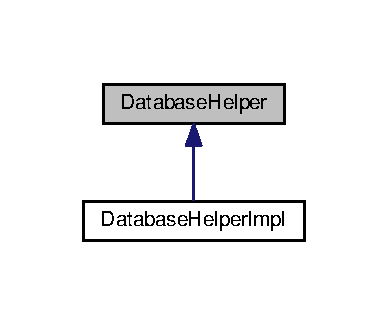
\includegraphics[width=186pt]{d0/dc0/classDatabaseHelper__inherit__graph}
\end{center}
\end{figure}
\subsection*{Public Member Functions}
\begin{DoxyCompactItemize}
\item 
virtual int \hyperlink{classDatabaseHelper_a03e499b83f152466abed94fef2f0ef73}{get\+User\+Id} (Q\+String username)=0
\begin{DoxyCompactList}\small\item\em Esse método busca se um usuário está presente no banco de dados. \end{DoxyCompactList}\item 
virtual bool \hyperlink{classDatabaseHelper_aaff1d6157ea2d4fa7edb6744e8ce7daf}{insert\+Operation} (int user\+Id, double v1, Q\+String operacao, double v2, double resultado)=0
\begin{DoxyCompactList}\small\item\em Esse método armazena um registro de operação. \end{DoxyCompactList}\item 
virtual vector$<$ pair$<$ Q\+String, Q\+String $>$ $>$ \hyperlink{classDatabaseHelper_a32fe64f07291bbefc59e92690b7017bf}{get\+All\+Users} ()=0
\begin{DoxyCompactList}\small\item\em Retorna todos os usuários do banco e seus respectivas senhas. \end{DoxyCompactList}\item 
virtual vector$<$ pair$<$ Q\+String, int $>$ $>$ \hyperlink{classDatabaseHelper_ae9b9e741f7a776348dd334de3fa7e52b}{get\+Operations\+By\+User} (Q\+String username)=0
\begin{DoxyCompactList}\small\item\em Gera uma tabela de sobre as operações realizadas pelo usuário. \end{DoxyCompactList}\item 
virtual vector$<$ pair$<$ Q\+String, int $>$ $>$ \hyperlink{classDatabaseHelper_adc20c023d6dd87602bfd3310bddcf6d1}{get\+All\+Operations} ()=0
\begin{DoxyCompactList}\small\item\em Gera uma tabela de sobre as operações realizadas por todos os usuários. \end{DoxyCompactList}\item 
virtual bool \hyperlink{classDatabaseHelper_aca0024be103d394caf3a6eef7899c714}{is\+Admin} (Q\+String username)=0
\begin{DoxyCompactList}\small\item\em Verifica se um usuário tem permissõe de administrador. \end{DoxyCompactList}\end{DoxyCompactItemize}


\subsection{Detailed Description}
Interface para acesso a um banco de dados. 

\subsection{Member Function Documentation}
\index{Database\+Helper@{Database\+Helper}!get\+All\+Operations@{get\+All\+Operations}}
\index{get\+All\+Operations@{get\+All\+Operations}!Database\+Helper@{Database\+Helper}}
\subsubsection[{\texorpdfstring{get\+All\+Operations()=0}{getAllOperations()=0}}]{\setlength{\rightskip}{0pt plus 5cm}virtual vector$<$pair$<$Q\+String, int$>$ $>$ Database\+Helper\+::get\+All\+Operations (
\begin{DoxyParamCaption}
{}
\end{DoxyParamCaption}
)\hspace{0.3cm}{\ttfamily [pure virtual]}}\hypertarget{classDatabaseHelper_adc20c023d6dd87602bfd3310bddcf6d1}{}\label{classDatabaseHelper_adc20c023d6dd87602bfd3310bddcf6d1}


Gera uma tabela de sobre as operações realizadas por todos os usuários. 

\begin{DoxyReturn}{Returns}
Lista de pares contendo tipo de operação e quantidade de vezes que ela foi realizada. 
\end{DoxyReturn}
\begin{DoxySeeAlso}{See also}
\hyperlink{classDatabaseHelper_ae9b9e741f7a776348dd334de3fa7e52b}{Database\+Helper\+::get\+Operations\+By\+User(\+Q\+String)}. 
\end{DoxySeeAlso}


Implemented in \hyperlink{classDatabaseHelperImpl_aedd37d515fad4f0b0884748bf77f677c}{Database\+Helper\+Impl}.

\index{Database\+Helper@{Database\+Helper}!get\+All\+Users@{get\+All\+Users}}
\index{get\+All\+Users@{get\+All\+Users}!Database\+Helper@{Database\+Helper}}
\subsubsection[{\texorpdfstring{get\+All\+Users()=0}{getAllUsers()=0}}]{\setlength{\rightskip}{0pt plus 5cm}virtual vector$<$pair$<$Q\+String, Q\+String$>$ $>$ Database\+Helper\+::get\+All\+Users (
\begin{DoxyParamCaption}
{}
\end{DoxyParamCaption}
)\hspace{0.3cm}{\ttfamily [pure virtual]}}\hypertarget{classDatabaseHelper_a32fe64f07291bbefc59e92690b7017bf}{}\label{classDatabaseHelper_a32fe64f07291bbefc59e92690b7017bf}


Retorna todos os usuários do banco e seus respectivas senhas. 

\begin{DoxyReturn}{Returns}
Lista de pares contendo nome de usuário e senha. 
\end{DoxyReturn}


Implemented in \hyperlink{classDatabaseHelperImpl_ac93f23c05d794595149585c451f24605}{Database\+Helper\+Impl}.

\index{Database\+Helper@{Database\+Helper}!get\+Operations\+By\+User@{get\+Operations\+By\+User}}
\index{get\+Operations\+By\+User@{get\+Operations\+By\+User}!Database\+Helper@{Database\+Helper}}
\subsubsection[{\texorpdfstring{get\+Operations\+By\+User(\+Q\+String username)=0}{getOperationsByUser(QString username)=0}}]{\setlength{\rightskip}{0pt plus 5cm}virtual vector$<$pair$<$Q\+String, int$>$ $>$ Database\+Helper\+::get\+Operations\+By\+User (
\begin{DoxyParamCaption}
\item[{Q\+String}]{username}
\end{DoxyParamCaption}
)\hspace{0.3cm}{\ttfamily [pure virtual]}}\hypertarget{classDatabaseHelper_ae9b9e741f7a776348dd334de3fa7e52b}{}\label{classDatabaseHelper_ae9b9e741f7a776348dd334de3fa7e52b}


Gera uma tabela de sobre as operações realizadas pelo usuário. 


\begin{DoxyParams}{Parameters}
{\em username} & Nome do usuário a ser buscado. \\
\hline
\end{DoxyParams}
\begin{DoxyReturn}{Returns}
Lista de pares contendo tipo de operação e quantidade de vezes que ela foi realizada. 
\end{DoxyReturn}
\begin{DoxySeeAlso}{See also}
\hyperlink{classDatabaseHelper_adc20c023d6dd87602bfd3310bddcf6d1}{Database\+Helper\+::get\+All\+Operations()}. 
\end{DoxySeeAlso}


Implemented in \hyperlink{classDatabaseHelperImpl_a124bd600c3e2daa19dc24982eb3dea14}{Database\+Helper\+Impl}.

\index{Database\+Helper@{Database\+Helper}!get\+User\+Id@{get\+User\+Id}}
\index{get\+User\+Id@{get\+User\+Id}!Database\+Helper@{Database\+Helper}}
\subsubsection[{\texorpdfstring{get\+User\+Id(\+Q\+String username)=0}{getUserId(QString username)=0}}]{\setlength{\rightskip}{0pt plus 5cm}virtual int Database\+Helper\+::get\+User\+Id (
\begin{DoxyParamCaption}
\item[{Q\+String}]{username}
\end{DoxyParamCaption}
)\hspace{0.3cm}{\ttfamily [pure virtual]}}\hypertarget{classDatabaseHelper_a03e499b83f152466abed94fef2f0ef73}{}\label{classDatabaseHelper_a03e499b83f152466abed94fef2f0ef73}


Esse método busca se um usuário está presente no banco de dados. 


\begin{DoxyParams}{Parameters}
{\em username} & Nome do usuário a ser buscado. \\
\hline
\end{DoxyParams}
\begin{DoxyReturn}{Returns}
O id do usuário no banco. 
\end{DoxyReturn}


Implemented in \hyperlink{classDatabaseHelperImpl_a071ca71dc50d21a3d5749156aec99476}{Database\+Helper\+Impl}.

\index{Database\+Helper@{Database\+Helper}!insert\+Operation@{insert\+Operation}}
\index{insert\+Operation@{insert\+Operation}!Database\+Helper@{Database\+Helper}}
\subsubsection[{\texorpdfstring{insert\+Operation(int user\+Id, double v1, Q\+String operacao, double v2, double resultado)=0}{insertOperation(int userId, double v1, QString operacao, double v2, double resultado)=0}}]{\setlength{\rightskip}{0pt plus 5cm}virtual bool Database\+Helper\+::insert\+Operation (
\begin{DoxyParamCaption}
\item[{int}]{user\+Id, }
\item[{double}]{v1, }
\item[{Q\+String}]{operacao, }
\item[{double}]{v2, }
\item[{double}]{resultado}
\end{DoxyParamCaption}
)\hspace{0.3cm}{\ttfamily [pure virtual]}}\hypertarget{classDatabaseHelper_aaff1d6157ea2d4fa7edb6744e8ce7daf}{}\label{classDatabaseHelper_aaff1d6157ea2d4fa7edb6744e8ce7daf}


Esse método armazena um registro de operação. 


\begin{DoxyParams}{Parameters}
{\em user\+Id} & Id do usuário que realizou a operação. \\
\hline
{\em v1} & Primeiro operando. \\
\hline
{\em operacao} & Operação realizada. \\
\hline
{\em v2} & Segundo Operando. \\
\hline
{\em resultado} & Resultado da operação. \\
\hline
\end{DoxyParams}
\begin{DoxyReturn}{Returns}
Se a inserção foi realizada. 
\end{DoxyReturn}


Implemented in \hyperlink{classDatabaseHelperImpl_a4791d584b178b71a186a843dbc8ab86e}{Database\+Helper\+Impl}.

\index{Database\+Helper@{Database\+Helper}!is\+Admin@{is\+Admin}}
\index{is\+Admin@{is\+Admin}!Database\+Helper@{Database\+Helper}}
\subsubsection[{\texorpdfstring{is\+Admin(\+Q\+String username)=0}{isAdmin(QString username)=0}}]{\setlength{\rightskip}{0pt plus 5cm}virtual bool Database\+Helper\+::is\+Admin (
\begin{DoxyParamCaption}
\item[{Q\+String}]{username}
\end{DoxyParamCaption}
)\hspace{0.3cm}{\ttfamily [pure virtual]}}\hypertarget{classDatabaseHelper_aca0024be103d394caf3a6eef7899c714}{}\label{classDatabaseHelper_aca0024be103d394caf3a6eef7899c714}


Verifica se um usuário tem permissõe de administrador. 


\begin{DoxyParams}{Parameters}
{\em username} & Nome do usuário a ser buscado. \\
\hline
\end{DoxyParams}
\begin{DoxyReturn}{Returns}
Se o usuário é administrador. 
\end{DoxyReturn}


Implemented in \hyperlink{classDatabaseHelperImpl_a3c6da9438b26955fcef6a080c85652f5}{Database\+Helper\+Impl}.



The documentation for this class was generated from the following file\+:\begin{DoxyCompactItemize}
\item 
Calc\+Server/src/database/\hyperlink{databasehelper_8h}{databasehelper.\+h}\end{DoxyCompactItemize}

\hypertarget{classDatabaseHelperImpl}{}\section{Database\+Helper\+Impl Class Reference}
\label{classDatabaseHelperImpl}\index{Database\+Helper\+Impl@{Database\+Helper\+Impl}}


Implementação da Interface \hyperlink{classDatabaseHelper}{Database\+Helper} para acesso ao banco de dados S\+Q\+Lite.  




{\ttfamily \#include $<$databasehelperimpl.\+h$>$}



Inheritance diagram for Database\+Helper\+Impl\+:\nopagebreak
\begin{figure}[H]
\begin{center}
\leavevmode
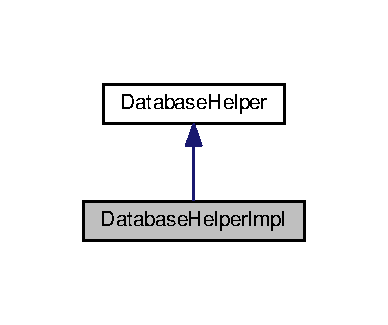
\includegraphics[width=186pt]{dd/d1d/classDatabaseHelperImpl__inherit__graph}
\end{center}
\end{figure}


Collaboration diagram for Database\+Helper\+Impl\+:\nopagebreak
\begin{figure}[H]
\begin{center}
\leavevmode
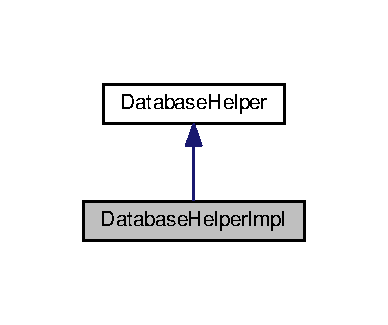
\includegraphics[width=186pt]{d8/da4/classDatabaseHelperImpl__coll__graph}
\end{center}
\end{figure}
\subsection*{Public Member Functions}
\begin{DoxyCompactItemize}
\item 
\hyperlink{classDatabaseHelperImpl_a60f67f9c6183e02ffab826bf254fef10}{Database\+Helper\+Impl} ()\hypertarget{classDatabaseHelperImpl_a60f67f9c6183e02ffab826bf254fef10}{}\label{classDatabaseHelperImpl_a60f67f9c6183e02ffab826bf254fef10}

\begin{DoxyCompactList}\small\item\em Construtor padrão. \end{DoxyCompactList}\item 
virtual \hyperlink{classDatabaseHelperImpl_a14d7fa4590316828d2e802bff3512223}{$\sim$\+Database\+Helper\+Impl} ()\hypertarget{classDatabaseHelperImpl_a14d7fa4590316828d2e802bff3512223}{}\label{classDatabaseHelperImpl_a14d7fa4590316828d2e802bff3512223}

\begin{DoxyCompactList}\small\item\em Destrutor padrão. \end{DoxyCompactList}\item 
virtual int \hyperlink{classDatabaseHelperImpl_a071ca71dc50d21a3d5749156aec99476}{get\+User\+Id} (Q\+String username)
\begin{DoxyCompactList}\small\item\em Esse método busca se um usuário está presente no banco de dados. \end{DoxyCompactList}\item 
virtual bool \hyperlink{classDatabaseHelperImpl_a4791d584b178b71a186a843dbc8ab86e}{insert\+Operation} (int user\+Id, double v1, Q\+String operacao, double v2, double resultado)
\begin{DoxyCompactList}\small\item\em Esse método armazena um registro de operação. \end{DoxyCompactList}\item 
virtual vector$<$ pair$<$ Q\+String, Q\+String $>$ $>$ \hyperlink{classDatabaseHelperImpl_ac93f23c05d794595149585c451f24605}{get\+All\+Users} ()
\begin{DoxyCompactList}\small\item\em Retorna todos os usuários do banco e seus respectivas senhas. \end{DoxyCompactList}\item 
virtual vector$<$ pair$<$ Q\+String, int $>$ $>$ \hyperlink{classDatabaseHelperImpl_a124bd600c3e2daa19dc24982eb3dea14}{get\+Operations\+By\+User} (Q\+String username)
\begin{DoxyCompactList}\small\item\em Gera uma tabela de sobre as operações realizadas pelo usuário. \end{DoxyCompactList}\item 
virtual vector$<$ pair$<$ Q\+String, int $>$ $>$ \hyperlink{classDatabaseHelperImpl_aedd37d515fad4f0b0884748bf77f677c}{get\+All\+Operations} ()
\begin{DoxyCompactList}\small\item\em Gera uma tabela de sobre as operações realizadas por todos os usuários. \end{DoxyCompactList}\item 
virtual bool \hyperlink{classDatabaseHelperImpl_a3c6da9438b26955fcef6a080c85652f5}{is\+Admin} (Q\+String username)
\begin{DoxyCompactList}\small\item\em Verifica se um usuário tem permissõe de administrador. \end{DoxyCompactList}\end{DoxyCompactItemize}
\subsection*{Protected Attributes}
\begin{DoxyCompactItemize}
\item 
Q\+Sql\+Database \hyperlink{classDatabaseHelperImpl_a0bc1ee11321daa34b2abe7306c6184c2}{sql\+Database}\hypertarget{classDatabaseHelperImpl_a0bc1ee11321daa34b2abe7306c6184c2}{}\label{classDatabaseHelperImpl_a0bc1ee11321daa34b2abe7306c6184c2}

\begin{DoxyCompactList}\small\item\em Objeto de gerenciamento do banco de dados. \end{DoxyCompactList}\end{DoxyCompactItemize}
\subsection*{Private Member Functions}
\begin{DoxyCompactItemize}
\item 
\hyperlink{classDatabaseHelperImpl_a88e80bd1c92b35e3e8a4fe1238215245}{Database\+Helper\+Impl} (const \hyperlink{classDatabaseHelperImpl}{Database\+Helper\+Impl} \&rhs)
\begin{DoxyCompactList}\small\item\em Construtor de Cópia. \end{DoxyCompactList}\item 
\hyperlink{classDatabaseHelperImpl}{Database\+Helper\+Impl} \& \hyperlink{classDatabaseHelperImpl_a48022ad027303dc93626f3293887b98e}{operator=} (const \hyperlink{classDatabaseHelperImpl}{Database\+Helper\+Impl} \&rhs)
\begin{DoxyCompactList}\small\item\em Sobrecarga do operador =. \end{DoxyCompactList}\item 
void \hyperlink{classDatabaseHelperImpl_af1b1b1496a9027cd09ee0456010ad9bd}{setup\+Database} ()
\begin{DoxyCompactList}\small\item\em Metódo para inicialização do banco de dados. \end{DoxyCompactList}\end{DoxyCompactItemize}
\subsection*{Friends}
\begin{DoxyCompactItemize}
\item 
class \hyperlink{classDatabaseHelperImpl_adebc71025cd8245ef1624f16ffbca46b}{Database\+Helper\+Impl\+Test}\hypertarget{classDatabaseHelperImpl_adebc71025cd8245ef1624f16ffbca46b}{}\label{classDatabaseHelperImpl_adebc71025cd8245ef1624f16ffbca46b}

\begin{DoxyCompactList}\small\item\em Classe de Testes para \hyperlink{classDatabaseHelperImpl}{Database\+Helper\+Impl}. \end{DoxyCompactList}\end{DoxyCompactItemize}


\subsection{Detailed Description}
Implementação da Interface \hyperlink{classDatabaseHelper}{Database\+Helper} para acesso ao banco de dados S\+Q\+Lite. 

\subsection{Constructor \& Destructor Documentation}
\index{Database\+Helper\+Impl@{Database\+Helper\+Impl}!Database\+Helper\+Impl@{Database\+Helper\+Impl}}
\index{Database\+Helper\+Impl@{Database\+Helper\+Impl}!Database\+Helper\+Impl@{Database\+Helper\+Impl}}
\subsubsection[{\texorpdfstring{Database\+Helper\+Impl(const Database\+Helper\+Impl \&rhs)}{DatabaseHelperImpl(const DatabaseHelperImpl &rhs)}}]{\setlength{\rightskip}{0pt plus 5cm}Database\+Helper\+Impl\+::\+Database\+Helper\+Impl (
\begin{DoxyParamCaption}
\item[{const {\bf Database\+Helper\+Impl} \&}]{rhs}
\end{DoxyParamCaption}
)\hspace{0.3cm}{\ttfamily [private]}}\hypertarget{classDatabaseHelperImpl_a88e80bd1c92b35e3e8a4fe1238215245}{}\label{classDatabaseHelperImpl_a88e80bd1c92b35e3e8a4fe1238215245}


Construtor de Cópia. 


\begin{DoxyParams}{Parameters}
{\em rhs} & Objeto a ser copiado. \\
\hline
\end{DoxyParams}


\subsection{Member Function Documentation}
\index{Database\+Helper\+Impl@{Database\+Helper\+Impl}!get\+All\+Operations@{get\+All\+Operations}}
\index{get\+All\+Operations@{get\+All\+Operations}!Database\+Helper\+Impl@{Database\+Helper\+Impl}}
\subsubsection[{\texorpdfstring{get\+All\+Operations()}{getAllOperations()}}]{\setlength{\rightskip}{0pt plus 5cm}vector$<$ pair$<$ Q\+String, int $>$ $>$ Database\+Helper\+Impl\+::get\+All\+Operations (
\begin{DoxyParamCaption}
{}
\end{DoxyParamCaption}
)\hspace{0.3cm}{\ttfamily [virtual]}}\hypertarget{classDatabaseHelperImpl_aedd37d515fad4f0b0884748bf77f677c}{}\label{classDatabaseHelperImpl_aedd37d515fad4f0b0884748bf77f677c}


Gera uma tabela de sobre as operações realizadas por todos os usuários. 

\begin{DoxyReturn}{Returns}
Lista de pares contendo tipo de operação e quantidade de vezes que ela foi realizada. 
\end{DoxyReturn}
\begin{DoxySeeAlso}{See also}
\hyperlink{classDatabaseHelper_ae9b9e741f7a776348dd334de3fa7e52b}{Database\+Helper\+::get\+Operations\+By\+User(\+Q\+String)}. 
\end{DoxySeeAlso}


Implements \hyperlink{classDatabaseHelper_adc20c023d6dd87602bfd3310bddcf6d1}{Database\+Helper}.

\index{Database\+Helper\+Impl@{Database\+Helper\+Impl}!get\+All\+Users@{get\+All\+Users}}
\index{get\+All\+Users@{get\+All\+Users}!Database\+Helper\+Impl@{Database\+Helper\+Impl}}
\subsubsection[{\texorpdfstring{get\+All\+Users()}{getAllUsers()}}]{\setlength{\rightskip}{0pt plus 5cm}vector$<$ pair$<$ Q\+String, Q\+String $>$ $>$ Database\+Helper\+Impl\+::get\+All\+Users (
\begin{DoxyParamCaption}
{}
\end{DoxyParamCaption}
)\hspace{0.3cm}{\ttfamily [virtual]}}\hypertarget{classDatabaseHelperImpl_ac93f23c05d794595149585c451f24605}{}\label{classDatabaseHelperImpl_ac93f23c05d794595149585c451f24605}


Retorna todos os usuários do banco e seus respectivas senhas. 

\begin{DoxyReturn}{Returns}
Lista de pares contendo nome de usuário e senha. 
\end{DoxyReturn}


Implements \hyperlink{classDatabaseHelper_a32fe64f07291bbefc59e92690b7017bf}{Database\+Helper}.

\index{Database\+Helper\+Impl@{Database\+Helper\+Impl}!get\+Operations\+By\+User@{get\+Operations\+By\+User}}
\index{get\+Operations\+By\+User@{get\+Operations\+By\+User}!Database\+Helper\+Impl@{Database\+Helper\+Impl}}
\subsubsection[{\texorpdfstring{get\+Operations\+By\+User(\+Q\+String username)}{getOperationsByUser(QString username)}}]{\setlength{\rightskip}{0pt plus 5cm}vector$<$ pair$<$ Q\+String, int $>$ $>$ Database\+Helper\+Impl\+::get\+Operations\+By\+User (
\begin{DoxyParamCaption}
\item[{Q\+String}]{username}
\end{DoxyParamCaption}
)\hspace{0.3cm}{\ttfamily [virtual]}}\hypertarget{classDatabaseHelperImpl_a124bd600c3e2daa19dc24982eb3dea14}{}\label{classDatabaseHelperImpl_a124bd600c3e2daa19dc24982eb3dea14}


Gera uma tabela de sobre as operações realizadas pelo usuário. 


\begin{DoxyParams}{Parameters}
{\em username} & Nome do usuário a ser buscado. \\
\hline
\end{DoxyParams}
\begin{DoxyReturn}{Returns}
Lista de pares contendo tipo de operação e quantidade de vezes que ela foi realizada. 
\end{DoxyReturn}
\begin{DoxySeeAlso}{See also}
\hyperlink{classDatabaseHelper_adc20c023d6dd87602bfd3310bddcf6d1}{Database\+Helper\+::get\+All\+Operations()}. 
\end{DoxySeeAlso}


Implements \hyperlink{classDatabaseHelper_ae9b9e741f7a776348dd334de3fa7e52b}{Database\+Helper}.

\index{Database\+Helper\+Impl@{Database\+Helper\+Impl}!get\+User\+Id@{get\+User\+Id}}
\index{get\+User\+Id@{get\+User\+Id}!Database\+Helper\+Impl@{Database\+Helper\+Impl}}
\subsubsection[{\texorpdfstring{get\+User\+Id(\+Q\+String username)}{getUserId(QString username)}}]{\setlength{\rightskip}{0pt plus 5cm}int Database\+Helper\+Impl\+::get\+User\+Id (
\begin{DoxyParamCaption}
\item[{Q\+String}]{username}
\end{DoxyParamCaption}
)\hspace{0.3cm}{\ttfamily [virtual]}}\hypertarget{classDatabaseHelperImpl_a071ca71dc50d21a3d5749156aec99476}{}\label{classDatabaseHelperImpl_a071ca71dc50d21a3d5749156aec99476}


Esse método busca se um usuário está presente no banco de dados. 


\begin{DoxyParams}{Parameters}
{\em username} & Nome do usuário a ser buscado. \\
\hline
\end{DoxyParams}
\begin{DoxyReturn}{Returns}
O id do usuário no banco. 
\end{DoxyReturn}


Implements \hyperlink{classDatabaseHelper_a03e499b83f152466abed94fef2f0ef73}{Database\+Helper}.

\index{Database\+Helper\+Impl@{Database\+Helper\+Impl}!insert\+Operation@{insert\+Operation}}
\index{insert\+Operation@{insert\+Operation}!Database\+Helper\+Impl@{Database\+Helper\+Impl}}
\subsubsection[{\texorpdfstring{insert\+Operation(int user\+Id, double v1, Q\+String operacao, double v2, double resultado)}{insertOperation(int userId, double v1, QString operacao, double v2, double resultado)}}]{\setlength{\rightskip}{0pt plus 5cm}bool Database\+Helper\+Impl\+::insert\+Operation (
\begin{DoxyParamCaption}
\item[{int}]{user\+Id, }
\item[{double}]{v1, }
\item[{Q\+String}]{operacao, }
\item[{double}]{v2, }
\item[{double}]{resultado}
\end{DoxyParamCaption}
)\hspace{0.3cm}{\ttfamily [virtual]}}\hypertarget{classDatabaseHelperImpl_a4791d584b178b71a186a843dbc8ab86e}{}\label{classDatabaseHelperImpl_a4791d584b178b71a186a843dbc8ab86e}


Esse método armazena um registro de operação. 


\begin{DoxyParams}{Parameters}
{\em user\+Id} & Id do usuário que realizou a operação. \\
\hline
{\em v1} & Primeiro operando. \\
\hline
{\em operacao} & Operação realizada. \\
\hline
{\em v2} & Segundo Operando. \\
\hline
{\em resultado} & Resultado da operação. \\
\hline
\end{DoxyParams}
\begin{DoxyReturn}{Returns}
Se a inserção foi realizada. 
\end{DoxyReturn}


Implements \hyperlink{classDatabaseHelper_aaff1d6157ea2d4fa7edb6744e8ce7daf}{Database\+Helper}.

\index{Database\+Helper\+Impl@{Database\+Helper\+Impl}!is\+Admin@{is\+Admin}}
\index{is\+Admin@{is\+Admin}!Database\+Helper\+Impl@{Database\+Helper\+Impl}}
\subsubsection[{\texorpdfstring{is\+Admin(\+Q\+String username)}{isAdmin(QString username)}}]{\setlength{\rightskip}{0pt plus 5cm}bool Database\+Helper\+Impl\+::is\+Admin (
\begin{DoxyParamCaption}
\item[{Q\+String}]{username}
\end{DoxyParamCaption}
)\hspace{0.3cm}{\ttfamily [virtual]}}\hypertarget{classDatabaseHelperImpl_a3c6da9438b26955fcef6a080c85652f5}{}\label{classDatabaseHelperImpl_a3c6da9438b26955fcef6a080c85652f5}


Verifica se um usuário tem permissõe de administrador. 


\begin{DoxyParams}{Parameters}
{\em username} & Nome do usuário a ser buscado. \\
\hline
\end{DoxyParams}
\begin{DoxyReturn}{Returns}
Se o usuário é administrador. 
\end{DoxyReturn}


Implements \hyperlink{classDatabaseHelper_aca0024be103d394caf3a6eef7899c714}{Database\+Helper}.

\index{Database\+Helper\+Impl@{Database\+Helper\+Impl}!operator=@{operator=}}
\index{operator=@{operator=}!Database\+Helper\+Impl@{Database\+Helper\+Impl}}
\subsubsection[{\texorpdfstring{operator=(const Database\+Helper\+Impl \&rhs)}{operator=(const DatabaseHelperImpl &rhs)}}]{\setlength{\rightskip}{0pt plus 5cm}{\bf Database\+Helper\+Impl} \& Database\+Helper\+Impl\+::operator= (
\begin{DoxyParamCaption}
\item[{const {\bf Database\+Helper\+Impl} \&}]{rhs}
\end{DoxyParamCaption}
)\hspace{0.3cm}{\ttfamily [private]}}\hypertarget{classDatabaseHelperImpl_a48022ad027303dc93626f3293887b98e}{}\label{classDatabaseHelperImpl_a48022ad027303dc93626f3293887b98e}


Sobrecarga do operador =. 


\begin{DoxyParams}{Parameters}
{\em rhs} & Objeto a ser copiado. \\
\hline
\end{DoxyParams}
\begin{DoxyReturn}{Returns}
Novo objeto copiado. 
\end{DoxyReturn}
\index{Database\+Helper\+Impl@{Database\+Helper\+Impl}!setup\+Database@{setup\+Database}}
\index{setup\+Database@{setup\+Database}!Database\+Helper\+Impl@{Database\+Helper\+Impl}}
\subsubsection[{\texorpdfstring{setup\+Database()}{setupDatabase()}}]{\setlength{\rightskip}{0pt plus 5cm}void Database\+Helper\+Impl\+::setup\+Database (
\begin{DoxyParamCaption}
{}
\end{DoxyParamCaption}
)\hspace{0.3cm}{\ttfamily [private]}}\hypertarget{classDatabaseHelperImpl_af1b1b1496a9027cd09ee0456010ad9bd}{}\label{classDatabaseHelperImpl_af1b1b1496a9027cd09ee0456010ad9bd}


Metódo para inicialização do banco de dados. 

Este método configura o gerenciador de banco de dados para trabalhar com o drive Q\+S\+Q\+L\+I\+TE e a instância do banco nomeada calc\+\_\+example.\+sqlite. 

The documentation for this class was generated from the following files\+:\begin{DoxyCompactItemize}
\item 
Calc\+Server/\hyperlink{databasehelperimpl_8h}{databasehelperimpl.\+h}\item 
Calc\+Server/\hyperlink{databasehelperimpl_8cpp}{databasehelperimpl.\+cpp}\end{DoxyCompactItemize}

\hypertarget{classDialog}{}\section{Dialog Class Reference}
\label{classDialog}\index{Dialog@{Dialog}}


Classe para exibição dos dados do servidor.  




{\ttfamily \#include $<$dialog.\+h$>$}



Inheritance diagram for Dialog\+:\nopagebreak
\begin{figure}[H]
\begin{center}
\leavevmode
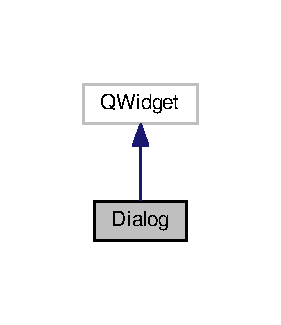
\includegraphics[width=135pt]{dc/de6/classDialog__inherit__graph}
\end{center}
\end{figure}


Collaboration diagram for Dialog\+:\nopagebreak
\begin{figure}[H]
\begin{center}
\leavevmode
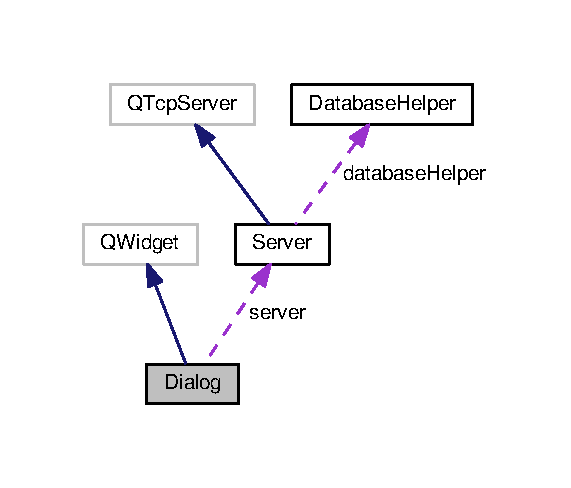
\includegraphics[width=274pt]{df/de8/classDialog__coll__graph}
\end{center}
\end{figure}
\subsection*{Public Member Functions}
\begin{DoxyCompactItemize}
\item 
\hyperlink{classDialog_acfa2063f9f962d394c6a645b6e7e08d8}{Dialog} (Q\+Widget $\ast$parent=0)
\begin{DoxyCompactList}\small\item\em Construtor padrão da classe \hyperlink{classDialog}{Dialog}. \end{DoxyCompactList}\end{DoxyCompactItemize}
\subsection*{Private Attributes}
\begin{DoxyCompactItemize}
\item 
Q\+Label $\ast$ \hyperlink{classDialog_a0637bc55b1a71b4667477778a8c72f9a}{status\+Label}\hypertarget{classDialog_a0637bc55b1a71b4667477778a8c72f9a}{}\label{classDialog_a0637bc55b1a71b4667477778a8c72f9a}

\begin{DoxyCompactList}\small\item\em Q\+Label para exibição dos dados do servidor. \end{DoxyCompactList}\item 
Q\+Push\+Button $\ast$ \hyperlink{classDialog_adad2ac3f09934c21fb4c797a88496376}{quit\+Button}\hypertarget{classDialog_adad2ac3f09934c21fb4c797a88496376}{}\label{classDialog_adad2ac3f09934c21fb4c797a88496376}

\begin{DoxyCompactList}\small\item\em Botão de sair da aplicação. \end{DoxyCompactList}\item 
\hyperlink{classServer}{Server} \hyperlink{classDialog_aec51788da8fed7e13ad1a66b8e0c4379}{server}\hypertarget{classDialog_aec51788da8fed7e13ad1a66b8e0c4379}{}\label{classDialog_aec51788da8fed7e13ad1a66b8e0c4379}

\begin{DoxyCompactList}\small\item\em Instância de \hyperlink{classServer}{Server}. \end{DoxyCompactList}\end{DoxyCompactItemize}
\subsection*{Friends}
\begin{DoxyCompactItemize}
\item 
class \hyperlink{classDialog_a9fe923be634f4d12f5a825141fafb85f}{Dialog\+Test}\hypertarget{classDialog_a9fe923be634f4d12f5a825141fafb85f}{}\label{classDialog_a9fe923be634f4d12f5a825141fafb85f}

\begin{DoxyCompactList}\small\item\em Classe de Testes para \hyperlink{classDialog}{Dialog}. \end{DoxyCompactList}\item 
class \hyperlink{classDialog_a9c408e8dbdb17dca5ff54b16daeed3f6}{Sockets\+Test}\hypertarget{classDialog_a9c408e8dbdb17dca5ff54b16daeed3f6}{}\label{classDialog_a9c408e8dbdb17dca5ff54b16daeed3f6}

\begin{DoxyCompactList}\small\item\em Classe de Testes para Sockets. \end{DoxyCompactList}\end{DoxyCompactItemize}


\subsection{Detailed Description}
Classe para exibição dos dados do servidor. 

Esta classe cria uma instância de \hyperlink{classServer}{Server} e exibe suas informações. 

\subsection{Constructor \& Destructor Documentation}
\index{Dialog@{Dialog}!Dialog@{Dialog}}
\index{Dialog@{Dialog}!Dialog@{Dialog}}
\subsubsection[{\texorpdfstring{Dialog(\+Q\+Widget $\ast$parent=0)}{Dialog(QWidget *parent=0)}}]{\setlength{\rightskip}{0pt plus 5cm}Dialog\+::\+Dialog (
\begin{DoxyParamCaption}
\item[{Q\+Widget $\ast$}]{parent = {\ttfamily 0}}
\end{DoxyParamCaption}
)}\hypertarget{classDialog_acfa2063f9f962d394c6a645b6e7e08d8}{}\label{classDialog_acfa2063f9f962d394c6a645b6e7e08d8}


Construtor padrão da classe \hyperlink{classDialog}{Dialog}. 

Instância e configura a interface. Além disso configura a instância de \hyperlink{classServer}{Server} antes de deixa-\/la tratando as requisições.


\begin{DoxyParams}{Parameters}
{\em parent} & Referência ao componente pai. \\
\hline
\end{DoxyParams}


The documentation for this class was generated from the following files\+:\begin{DoxyCompactItemize}
\item 
Calc\+Server/\hyperlink{dialog_8h}{dialog.\+h}\item 
Calc\+Server/\hyperlink{dialog_8cpp}{dialog.\+cpp}\end{DoxyCompactItemize}

\hypertarget{classMyCalcWindow}{}\section{My\+Calc\+Window Class Reference}
\label{classMyCalcWindow}\index{My\+Calc\+Window@{My\+Calc\+Window}}


Classe para gerenciar as ações de uma calculadora.  




{\ttfamily \#include $<$mycalcwindow.\+h$>$}



Inheritance diagram for My\+Calc\+Window\+:
\nopagebreak
\begin{figure}[H]
\begin{center}
\leavevmode
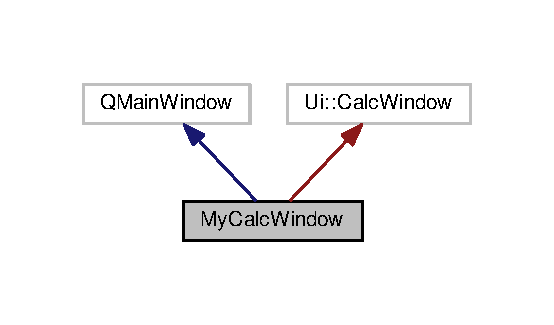
\includegraphics[width=266pt]{d9/d04/classMyCalcWindow__inherit__graph}
\end{center}
\end{figure}


Collaboration diagram for My\+Calc\+Window\+:
\nopagebreak
\begin{figure}[H]
\begin{center}
\leavevmode
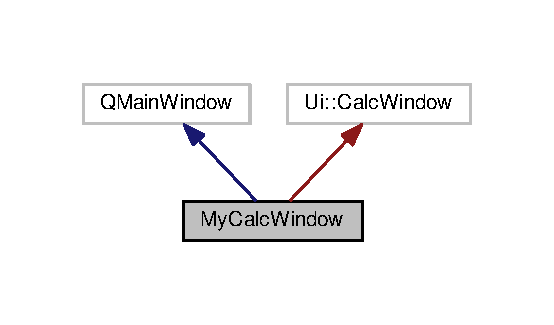
\includegraphics[width=322pt]{d6/dbc/classMyCalcWindow__coll__graph}
\end{center}
\end{figure}
\subsection*{Public Slots}
\begin{DoxyCompactItemize}
\item 
void \hyperlink{classMyCalcWindow_a6fdaf67619d3127503232c656e712656}{on\+\_\+exec\+Button\+\_\+clicked} (void)
\begin{DoxyCompactList}\small\item\em Slot chamado quando se clica no botão \textquotesingle{}Executar\textquotesingle{} e executa uma operação. \end{DoxyCompactList}\item 
void \hyperlink{classMyCalcWindow_ae1c714a5ad30c0fc67b9944481b30a05}{on\+\_\+radio\+Button\+Add\+\_\+clicked} (void)
\begin{DoxyCompactList}\small\item\em Slot chamado quando se clica no radio button da operação soma. \end{DoxyCompactList}\item 
void \hyperlink{classMyCalcWindow_a01fac328f5546feb830a67a7d35cc7f5}{on\+\_\+radio\+Button\+Sub\+\_\+clicked} (void)
\begin{DoxyCompactList}\small\item\em Slot chamado quando se clica no radio button da operação subtração. \end{DoxyCompactList}\item 
void \hyperlink{classMyCalcWindow_a553593de7766d99faf23a2053ddb4281}{on\+\_\+radio\+Button\+Mult\+\_\+clicked} (void)
\begin{DoxyCompactList}\small\item\em Slot chamado quando se clica no radio button da operação multiplicação. \end{DoxyCompactList}\item 
void \hyperlink{classMyCalcWindow_a1ac314ac5a743effc49465a295f796a4}{on\+\_\+radio\+Button\+Div\+\_\+clicked} (void)
\begin{DoxyCompactList}\small\item\em Slot chamado quando se clica no radio button da operação divisão. \end{DoxyCompactList}\item 
void \hyperlink{classMyCalcWindow_ad018832daea504f486bc1cb26f5cb0ec}{on\+\_\+action\+By\+User\+\_\+triggered} (void)
\begin{DoxyCompactList}\small\item\em Slot chamado quando selecionada a opção do menu \textquotesingle{}Por Usuário\textquotesingle{}. \end{DoxyCompactList}\item 
void \hyperlink{classMyCalcWindow_ab50a651bb1983993008960ad39d93ed6}{on\+\_\+action\+All\+Users\+\_\+triggered} (void)
\begin{DoxyCompactList}\small\item\em Slot chamado quando selecionada a opção do menu \textquotesingle{}Todos os Usuários\textquotesingle{}. \end{DoxyCompactList}\item 
void \hyperlink{classMyCalcWindow_ae563c8fa18e6d1c3a7c2c1014a133e66}{on\+\_\+user\+Role\+\_\+current\+Index\+Changed} (int)
\begin{DoxyCompactList}\small\item\em Método para delegar a atualização da interface dado uma mudança de papel do usuário. \end{DoxyCompactList}\item 
void \hyperlink{classMyCalcWindow_aa04caeaafdba97eeb25d3dd92be4d545}{on\+User\+Login} (\hyperlink{classUser}{User} $\ast$\hyperlink{classMyCalcWindow_a730189195d0831ae9fee62f7c519e439}{user})
\begin{DoxyCompactList}\small\item\em Slot chamado para se configurar a calculadora sobre informações de rede e usuário. \end{DoxyCompactList}\item 
void \hyperlink{classMyCalcWindow_a809b1da213d1424ba098c1f0ee2d0bd5}{on\+Quit} (void)\hypertarget{classMyCalcWindow_a809b1da213d1424ba098c1f0ee2d0bd5}{}\label{classMyCalcWindow_a809b1da213d1424ba098c1f0ee2d0bd5}

\begin{DoxyCompactList}\small\item\em Slot chamado ao se clicar no botão \textquotesingle{}Sair\textquotesingle{}. \end{DoxyCompactList}\item 
void \hyperlink{classMyCalcWindow_aaa868eba4e3ee5a52d28c0c34bbbd8cd}{read\+Message} (Q\+Json\+Object json\+Object)
\begin{DoxyCompactList}\small\item\em Slot chamado quando o socket recebe uma mensagem de resposta do servidor. \end{DoxyCompactList}\end{DoxyCompactItemize}
\subsection*{Public Member Functions}
\begin{DoxyCompactItemize}
\item 
\hyperlink{classMyCalcWindow_ac205ab2dbfbf802859774a090b066518}{My\+Calc\+Window} (Q\+Widget $\ast$parent=nullptr)
\begin{DoxyCompactList}\small\item\em Construtor Padrão para a classe \hyperlink{classMyCalcWindow}{My\+Calc\+Window}. \end{DoxyCompactList}\item 
virtual \hyperlink{classMyCalcWindow_a6226362b86860c067418d16b7da1e1e2}{$\sim$\+My\+Calc\+Window} ()
\begin{DoxyCompactList}\small\item\em Destrutor da classe \hyperlink{classMyCalcWindow}{My\+Calc\+Window}. \end{DoxyCompactList}\end{DoxyCompactItemize}
\subsection*{Private Member Functions}
\begin{DoxyCompactItemize}
\item 
void \hyperlink{classMyCalcWindow_a734b9dd51ee199d930855444695625c7}{execute} (void)
\begin{DoxyCompactList}\small\item\em Método privado para coleta dos dados e envio ao servidor para realização de operações. \end{DoxyCompactList}\item 
void \hyperlink{classMyCalcWindow_ade7d295cb55effe865349b7eef1a6d1a}{show\+Pie\+Chart} (Q\+String title, vector$<$ pair$<$ Q\+String, int $>$$>$ operations)
\begin{DoxyCompactList}\small\item\em Método é utilizado para se gerar exibições em gráfico pizza das operações realizadas, sejam por todos os usuários ou somente um deles. \end{DoxyCompactList}\item 
void \hyperlink{classMyCalcWindow_a9e1e6c80336ba383e2d2a8419446e1f9}{setup\+User\+Ui} (int role\+Code)
\begin{DoxyCompactList}\small\item\em Método para alterar a interface baseado no papel do usuário. \end{DoxyCompactList}\end{DoxyCompactItemize}
\subsection*{Private Attributes}
\begin{DoxyCompactItemize}
\item 
\hyperlink{classUser}{User} $\ast$ \hyperlink{classMyCalcWindow_a730189195d0831ae9fee62f7c519e439}{user}\hypertarget{classMyCalcWindow_a730189195d0831ae9fee62f7c519e439}{}\label{classMyCalcWindow_a730189195d0831ae9fee62f7c519e439}

\begin{DoxyCompactList}\small\item\em Referencia ao usuário da aplicação. \end{DoxyCompactList}\item 
Q\+Tcp\+Socket \hyperlink{classMyCalcWindow_aa07c81871dc4b11ab83324b544d66733}{tcp\+Socket}\hypertarget{classMyCalcWindow_aa07c81871dc4b11ab83324b544d66733}{}\label{classMyCalcWindow_aa07c81871dc4b11ab83324b544d66733}

\begin{DoxyCompactList}\small\item\em T\+C\+P\+Socket utilizado pela aplicação para comunicar com servidor. \end{DoxyCompactList}\item 
Q\+Main\+Window $\ast$ \hyperlink{classMyCalcWindow_a98ecf548e0cb3586ff4afc33bdfacb7a}{chart\+Window}\hypertarget{classMyCalcWindow_a98ecf548e0cb3586ff4afc33bdfacb7a}{}\label{classMyCalcWindow_a98ecf548e0cb3586ff4afc33bdfacb7a}

\begin{DoxyCompactList}\small\item\em Main\+Window auxiliar para exibição de gráficos de operações. \end{DoxyCompactList}\end{DoxyCompactItemize}
\subsection*{Static Private Attributes}
\begin{DoxyCompactItemize}
\item 
static const int \hyperlink{classMyCalcWindow_a5aad7da85f794398e01c5b553eff0fae}{U\+S\+ER} = 0\hypertarget{classMyCalcWindow_a5aad7da85f794398e01c5b553eff0fae}{}\label{classMyCalcWindow_a5aad7da85f794398e01c5b553eff0fae}

\begin{DoxyCompactList}\small\item\em Flag numerica representando o papel usuário. \end{DoxyCompactList}\item 
static const int \hyperlink{classMyCalcWindow_ac29d883c4ff53cc9d01c3e2add2fec52}{A\+D\+M\+IN} = 1\hypertarget{classMyCalcWindow_ac29d883c4ff53cc9d01c3e2add2fec52}{}\label{classMyCalcWindow_ac29d883c4ff53cc9d01c3e2add2fec52}

\begin{DoxyCompactList}\small\item\em Flag numerica representando o papel administrador. \end{DoxyCompactList}\end{DoxyCompactItemize}
\subsection*{Friends}
\begin{DoxyCompactItemize}
\item 
class \hyperlink{classMyCalcWindow_aec613ce0d143a48322f72a2b90819fcb}{My\+Login\+Dialog\+Test}\hypertarget{classMyCalcWindow_aec613ce0d143a48322f72a2b90819fcb}{}\label{classMyCalcWindow_aec613ce0d143a48322f72a2b90819fcb}

\begin{DoxyCompactList}\small\item\em Classe para Testes do \hyperlink{classMyLoginDialog}{My\+Login\+Dialog}. \end{DoxyCompactList}\item 
class \hyperlink{classMyCalcWindow_a5eaf2f81c93e423d3a80f10bd41e84f8}{My\+Calc\+Window\+Test}\hypertarget{classMyCalcWindow_a5eaf2f81c93e423d3a80f10bd41e84f8}{}\label{classMyCalcWindow_a5eaf2f81c93e423d3a80f10bd41e84f8}

\begin{DoxyCompactList}\small\item\em Classe para Testes do \hyperlink{classMyCalcWindow}{My\+Calc\+Window}. \end{DoxyCompactList}\end{DoxyCompactItemize}


\subsection{Detailed Description}
Classe para gerenciar as ações de uma calculadora. 

Esta classe gerencia as iterações do usuário com uma calculadora e delega todas suas operações a serem feitas no servidor. 

\subsection{Constructor \& Destructor Documentation}
\index{My\+Calc\+Window@{My\+Calc\+Window}!My\+Calc\+Window@{My\+Calc\+Window}}
\index{My\+Calc\+Window@{My\+Calc\+Window}!My\+Calc\+Window@{My\+Calc\+Window}}
\subsubsection[{\texorpdfstring{My\+Calc\+Window(\+Q\+Widget $\ast$parent=nullptr)}{MyCalcWindow(QWidget *parent=nullptr)}}]{\setlength{\rightskip}{0pt plus 5cm}My\+Calc\+Window\+::\+My\+Calc\+Window (
\begin{DoxyParamCaption}
\item[{Q\+Widget $\ast$}]{parent = {\ttfamily nullptr}}
\end{DoxyParamCaption}
)}\hypertarget{classMyCalcWindow_ac205ab2dbfbf802859774a090b066518}{}\label{classMyCalcWindow_ac205ab2dbfbf802859774a090b066518}


Construtor Padrão para a classe \hyperlink{classMyCalcWindow}{My\+Calc\+Window}. 

Esse construtor inicializa os atributos parent e chart\+Window. Além disso, o construtor configura a interface por meio do método \textquotesingle{}setup\+Ui\textquotesingle{} da classe pai Calc\+Window e conecta os slots para a leitura de mensagens do servidor e saída da aplicação.


\begin{DoxyParams}{Parameters}
{\em parent} & Referência ao componente pai. \\
\hline
\end{DoxyParams}
\index{My\+Calc\+Window@{My\+Calc\+Window}!````~My\+Calc\+Window@{$\sim$\+My\+Calc\+Window}}
\index{````~My\+Calc\+Window@{$\sim$\+My\+Calc\+Window}!My\+Calc\+Window@{My\+Calc\+Window}}
\subsubsection[{\texorpdfstring{$\sim$\+My\+Calc\+Window()}{~MyCalcWindow()}}]{\setlength{\rightskip}{0pt plus 5cm}My\+Calc\+Window\+::$\sim$\+My\+Calc\+Window (
\begin{DoxyParamCaption}
{}
\end{DoxyParamCaption}
)\hspace{0.3cm}{\ttfamily [virtual]}}\hypertarget{classMyCalcWindow_a6226362b86860c067418d16b7da1e1e2}{}\label{classMyCalcWindow_a6226362b86860c067418d16b7da1e1e2}


Destrutor da classe \hyperlink{classMyCalcWindow}{My\+Calc\+Window}. 

Esse destrutor é utilizado para deletar a referência contida em chart\+Window. 

\subsection{Member Function Documentation}
\index{My\+Calc\+Window@{My\+Calc\+Window}!execute@{execute}}
\index{execute@{execute}!My\+Calc\+Window@{My\+Calc\+Window}}
\subsubsection[{\texorpdfstring{execute(void)}{execute(void)}}]{\setlength{\rightskip}{0pt plus 5cm}void My\+Calc\+Window\+::execute (
\begin{DoxyParamCaption}
\item[{void}]{}
\end{DoxyParamCaption}
)\hspace{0.3cm}{\ttfamily [private]}}\hypertarget{classMyCalcWindow_a734b9dd51ee199d930855444695625c7}{}\label{classMyCalcWindow_a734b9dd51ee199d930855444695625c7}


Método privado para coleta dos dados e envio ao servidor para realização de operações. 

Este método extrai os dados da interface e solicita a execução da operação para o \hyperlink{classNetworkManager}{Network\+Manager}.

\begin{DoxySeeAlso}{See also}
\hyperlink{classMyCalcWindow_a6fdaf67619d3127503232c656e712656}{My\+Calc\+Window\+::on\+\_\+exec\+Button\+\_\+clicked()}, My\+Calc\+Window\+::on\+\_\+radio\+Button\+Soma\+\_\+clicked(), \hyperlink{classMyCalcWindow_a01fac328f5546feb830a67a7d35cc7f5}{My\+Calc\+Window\+::on\+\_\+radio\+Button\+Sub\+\_\+clicked()}, \hyperlink{classMyCalcWindow_a553593de7766d99faf23a2053ddb4281}{My\+Calc\+Window\+::on\+\_\+radio\+Button\+Mult\+\_\+clicked()}, \hyperlink{classMyCalcWindow_a1ac314ac5a743effc49465a295f796a4}{My\+Calc\+Window\+::on\+\_\+radio\+Button\+Div\+\_\+clicked()}, \hyperlink{classMyCalcWindow_aaa868eba4e3ee5a52d28c0c34bbbd8cd}{My\+Calc\+Window\+::read\+Message()}. 
\end{DoxySeeAlso}
\index{My\+Calc\+Window@{My\+Calc\+Window}!on\+\_\+action\+All\+Users\+\_\+triggered@{on\+\_\+action\+All\+Users\+\_\+triggered}}
\index{on\+\_\+action\+All\+Users\+\_\+triggered@{on\+\_\+action\+All\+Users\+\_\+triggered}!My\+Calc\+Window@{My\+Calc\+Window}}
\subsubsection[{\texorpdfstring{on\+\_\+action\+All\+Users\+\_\+triggered}{on_actionAllUsers_triggered}}]{\setlength{\rightskip}{0pt plus 5cm}void My\+Calc\+Window\+::on\+\_\+action\+All\+Users\+\_\+triggered (
\begin{DoxyParamCaption}
\item[{void}]{}
\end{DoxyParamCaption}
)\hspace{0.3cm}{\ttfamily [slot]}}\hypertarget{classMyCalcWindow_ab50a651bb1983993008960ad39d93ed6}{}\label{classMyCalcWindow_ab50a651bb1983993008960ad39d93ed6}


Slot chamado quando selecionada a opção do menu \textquotesingle{}Todos os Usuários\textquotesingle{}. 

Esse slot faz uma requisição ao \hyperlink{classNetworkManager}{Network\+Manager} dos dados de todas as operações realizadas por todos os usuários.

\begin{DoxySeeAlso}{See also}
\hyperlink{classMyCalcWindow_aaa868eba4e3ee5a52d28c0c34bbbd8cd}{My\+Calc\+Window\+::read\+Message()}, \hyperlink{classMyCalcWindow_ade7d295cb55effe865349b7eef1a6d1a}{My\+Calc\+Window\+::show\+Pie\+Chart(\+Q\+String, vector$<$pair$<$\+Q\+String, int$>$$>$)}. 
\end{DoxySeeAlso}
\index{My\+Calc\+Window@{My\+Calc\+Window}!on\+\_\+action\+By\+User\+\_\+triggered@{on\+\_\+action\+By\+User\+\_\+triggered}}
\index{on\+\_\+action\+By\+User\+\_\+triggered@{on\+\_\+action\+By\+User\+\_\+triggered}!My\+Calc\+Window@{My\+Calc\+Window}}
\subsubsection[{\texorpdfstring{on\+\_\+action\+By\+User\+\_\+triggered}{on_actionByUser_triggered}}]{\setlength{\rightskip}{0pt plus 5cm}void My\+Calc\+Window\+::on\+\_\+action\+By\+User\+\_\+triggered (
\begin{DoxyParamCaption}
\item[{void}]{}
\end{DoxyParamCaption}
)\hspace{0.3cm}{\ttfamily [slot]}}\hypertarget{classMyCalcWindow_ad018832daea504f486bc1cb26f5cb0ec}{}\label{classMyCalcWindow_ad018832daea504f486bc1cb26f5cb0ec}


Slot chamado quando selecionada a opção do menu \textquotesingle{}Por Usuário\textquotesingle{}. 

Esse slot faz uma requisição ao \hyperlink{classNetworkManager}{Network\+Manager} dos dados de todas as operações realizadas pelo usuário.

\begin{DoxySeeAlso}{See also}
\hyperlink{classMyCalcWindow_aaa868eba4e3ee5a52d28c0c34bbbd8cd}{My\+Calc\+Window\+::read\+Message()}, \hyperlink{classMyCalcWindow_ade7d295cb55effe865349b7eef1a6d1a}{My\+Calc\+Window\+::show\+Pie\+Chart(\+Q\+String, vector$<$pair$<$\+Q\+String, int$>$$>$)}. 
\end{DoxySeeAlso}
\index{My\+Calc\+Window@{My\+Calc\+Window}!on\+\_\+exec\+Button\+\_\+clicked@{on\+\_\+exec\+Button\+\_\+clicked}}
\index{on\+\_\+exec\+Button\+\_\+clicked@{on\+\_\+exec\+Button\+\_\+clicked}!My\+Calc\+Window@{My\+Calc\+Window}}
\subsubsection[{\texorpdfstring{on\+\_\+exec\+Button\+\_\+clicked}{on_execButton_clicked}}]{\setlength{\rightskip}{0pt plus 5cm}void My\+Calc\+Window\+::on\+\_\+exec\+Button\+\_\+clicked (
\begin{DoxyParamCaption}
\item[{void}]{}
\end{DoxyParamCaption}
)\hspace{0.3cm}{\ttfamily [slot]}}\hypertarget{classMyCalcWindow_a6fdaf67619d3127503232c656e712656}{}\label{classMyCalcWindow_a6fdaf67619d3127503232c656e712656}


Slot chamado quando se clica no botão \textquotesingle{}Executar\textquotesingle{} e executa uma operação. 

\begin{DoxySeeAlso}{See also}
\hyperlink{classMyCalcWindow_a734b9dd51ee199d930855444695625c7}{My\+Calc\+Window\+::execute()}. 
\end{DoxySeeAlso}
\index{My\+Calc\+Window@{My\+Calc\+Window}!on\+\_\+radio\+Button\+Add\+\_\+clicked@{on\+\_\+radio\+Button\+Add\+\_\+clicked}}
\index{on\+\_\+radio\+Button\+Add\+\_\+clicked@{on\+\_\+radio\+Button\+Add\+\_\+clicked}!My\+Calc\+Window@{My\+Calc\+Window}}
\subsubsection[{\texorpdfstring{on\+\_\+radio\+Button\+Add\+\_\+clicked}{on_radioButtonAdd_clicked}}]{\setlength{\rightskip}{0pt plus 5cm}void My\+Calc\+Window\+::on\+\_\+radio\+Button\+Add\+\_\+clicked (
\begin{DoxyParamCaption}
\item[{void}]{}
\end{DoxyParamCaption}
)\hspace{0.3cm}{\ttfamily [slot]}}\hypertarget{classMyCalcWindow_ae1c714a5ad30c0fc67b9944481b30a05}{}\label{classMyCalcWindow_ae1c714a5ad30c0fc67b9944481b30a05}


Slot chamado quando se clica no radio button da operação soma. 

\begin{DoxySeeAlso}{See also}
\hyperlink{classMyCalcWindow_a734b9dd51ee199d930855444695625c7}{My\+Calc\+Window\+::execute()}. 
\end{DoxySeeAlso}
\index{My\+Calc\+Window@{My\+Calc\+Window}!on\+\_\+radio\+Button\+Div\+\_\+clicked@{on\+\_\+radio\+Button\+Div\+\_\+clicked}}
\index{on\+\_\+radio\+Button\+Div\+\_\+clicked@{on\+\_\+radio\+Button\+Div\+\_\+clicked}!My\+Calc\+Window@{My\+Calc\+Window}}
\subsubsection[{\texorpdfstring{on\+\_\+radio\+Button\+Div\+\_\+clicked}{on_radioButtonDiv_clicked}}]{\setlength{\rightskip}{0pt plus 5cm}void My\+Calc\+Window\+::on\+\_\+radio\+Button\+Div\+\_\+clicked (
\begin{DoxyParamCaption}
\item[{void}]{}
\end{DoxyParamCaption}
)\hspace{0.3cm}{\ttfamily [slot]}}\hypertarget{classMyCalcWindow_a1ac314ac5a743effc49465a295f796a4}{}\label{classMyCalcWindow_a1ac314ac5a743effc49465a295f796a4}


Slot chamado quando se clica no radio button da operação divisão. 

\begin{DoxySeeAlso}{See also}
\hyperlink{classMyCalcWindow_a734b9dd51ee199d930855444695625c7}{My\+Calc\+Window\+::execute()}. 
\end{DoxySeeAlso}
\index{My\+Calc\+Window@{My\+Calc\+Window}!on\+\_\+radio\+Button\+Mult\+\_\+clicked@{on\+\_\+radio\+Button\+Mult\+\_\+clicked}}
\index{on\+\_\+radio\+Button\+Mult\+\_\+clicked@{on\+\_\+radio\+Button\+Mult\+\_\+clicked}!My\+Calc\+Window@{My\+Calc\+Window}}
\subsubsection[{\texorpdfstring{on\+\_\+radio\+Button\+Mult\+\_\+clicked}{on_radioButtonMult_clicked}}]{\setlength{\rightskip}{0pt plus 5cm}void My\+Calc\+Window\+::on\+\_\+radio\+Button\+Mult\+\_\+clicked (
\begin{DoxyParamCaption}
\item[{void}]{}
\end{DoxyParamCaption}
)\hspace{0.3cm}{\ttfamily [slot]}}\hypertarget{classMyCalcWindow_a553593de7766d99faf23a2053ddb4281}{}\label{classMyCalcWindow_a553593de7766d99faf23a2053ddb4281}


Slot chamado quando se clica no radio button da operação multiplicação. 

\begin{DoxySeeAlso}{See also}
\hyperlink{classMyCalcWindow_a734b9dd51ee199d930855444695625c7}{My\+Calc\+Window\+::execute()}. 
\end{DoxySeeAlso}
\index{My\+Calc\+Window@{My\+Calc\+Window}!on\+\_\+radio\+Button\+Sub\+\_\+clicked@{on\+\_\+radio\+Button\+Sub\+\_\+clicked}}
\index{on\+\_\+radio\+Button\+Sub\+\_\+clicked@{on\+\_\+radio\+Button\+Sub\+\_\+clicked}!My\+Calc\+Window@{My\+Calc\+Window}}
\subsubsection[{\texorpdfstring{on\+\_\+radio\+Button\+Sub\+\_\+clicked}{on_radioButtonSub_clicked}}]{\setlength{\rightskip}{0pt plus 5cm}void My\+Calc\+Window\+::on\+\_\+radio\+Button\+Sub\+\_\+clicked (
\begin{DoxyParamCaption}
\item[{void}]{}
\end{DoxyParamCaption}
)\hspace{0.3cm}{\ttfamily [slot]}}\hypertarget{classMyCalcWindow_a01fac328f5546feb830a67a7d35cc7f5}{}\label{classMyCalcWindow_a01fac328f5546feb830a67a7d35cc7f5}


Slot chamado quando se clica no radio button da operação subtração. 

\begin{DoxySeeAlso}{See also}
\hyperlink{classMyCalcWindow_a734b9dd51ee199d930855444695625c7}{My\+Calc\+Window\+::execute()}. 
\end{DoxySeeAlso}
\index{My\+Calc\+Window@{My\+Calc\+Window}!on\+\_\+user\+Role\+\_\+current\+Index\+Changed@{on\+\_\+user\+Role\+\_\+current\+Index\+Changed}}
\index{on\+\_\+user\+Role\+\_\+current\+Index\+Changed@{on\+\_\+user\+Role\+\_\+current\+Index\+Changed}!My\+Calc\+Window@{My\+Calc\+Window}}
\subsubsection[{\texorpdfstring{on\+\_\+user\+Role\+\_\+current\+Index\+Changed}{on_userRole_currentIndexChanged}}]{\setlength{\rightskip}{0pt plus 5cm}void My\+Calc\+Window\+::on\+\_\+user\+Role\+\_\+current\+Index\+Changed (
\begin{DoxyParamCaption}
\item[{int}]{position}
\end{DoxyParamCaption}
)\hspace{0.3cm}{\ttfamily [slot]}}\hypertarget{classMyCalcWindow_ae563c8fa18e6d1c3a7c2c1014a133e66}{}\label{classMyCalcWindow_ae563c8fa18e6d1c3a7c2c1014a133e66}


Método para delegar a atualização da interface dado uma mudança de papel do usuário. 


\begin{DoxyParams}{Parameters}
{\em position} & Opção selecionada no combo box \\
\hline
\end{DoxyParams}
\index{My\+Calc\+Window@{My\+Calc\+Window}!on\+User\+Login@{on\+User\+Login}}
\index{on\+User\+Login@{on\+User\+Login}!My\+Calc\+Window@{My\+Calc\+Window}}
\subsubsection[{\texorpdfstring{on\+User\+Login}{onUserLogin}}]{\setlength{\rightskip}{0pt plus 5cm}void My\+Calc\+Window\+::on\+User\+Login (
\begin{DoxyParamCaption}
\item[{{\bf User} $\ast$}]{user}
\end{DoxyParamCaption}
)\hspace{0.3cm}{\ttfamily [slot]}}\hypertarget{classMyCalcWindow_aa04caeaafdba97eeb25d3dd92be4d545}{}\label{classMyCalcWindow_aa04caeaafdba97eeb25d3dd92be4d545}


Slot chamado para se configurar a calculadora sobre informações de rede e usuário. 


\begin{DoxyParams}{Parameters}
{\em user} & Referencia ao usuário da aplicação. \\
\hline
\end{DoxyParams}
\index{My\+Calc\+Window@{My\+Calc\+Window}!read\+Message@{read\+Message}}
\index{read\+Message@{read\+Message}!My\+Calc\+Window@{My\+Calc\+Window}}
\subsubsection[{\texorpdfstring{read\+Message}{readMessage}}]{\setlength{\rightskip}{0pt plus 5cm}void My\+Calc\+Window\+::read\+Message (
\begin{DoxyParamCaption}
\item[{Q\+Json\+Object}]{json\+Object}
\end{DoxyParamCaption}
)\hspace{0.3cm}{\ttfamily [slot]}}\hypertarget{classMyCalcWindow_aaa868eba4e3ee5a52d28c0c34bbbd8cd}{}\label{classMyCalcWindow_aaa868eba4e3ee5a52d28c0c34bbbd8cd}


Slot chamado quando o socket recebe uma mensagem de resposta do servidor. 

Ao receber uma resposta do \hyperlink{classNetworkManager}{Network\+Manager}, este método extrai as informações da mensagem e realiza a operação correspondente.

\begin{DoxySeeAlso}{See also}
\hyperlink{classMyCalcWindow_a734b9dd51ee199d930855444695625c7}{My\+Calc\+Window\+::execute()}, \hyperlink{classMyCalcWindow_ab50a651bb1983993008960ad39d93ed6}{My\+Calc\+Window\+::on\+\_\+action\+All\+Users\+\_\+triggered()}, \hyperlink{classMyCalcWindow_ad018832daea504f486bc1cb26f5cb0ec}{My\+Calc\+Window\+::on\+\_\+action\+By\+User\+\_\+triggered()}. 
\end{DoxySeeAlso}
\index{My\+Calc\+Window@{My\+Calc\+Window}!setup\+User\+Ui@{setup\+User\+Ui}}
\index{setup\+User\+Ui@{setup\+User\+Ui}!My\+Calc\+Window@{My\+Calc\+Window}}
\subsubsection[{\texorpdfstring{setup\+User\+Ui(int role\+Code)}{setupUserUi(int roleCode)}}]{\setlength{\rightskip}{0pt plus 5cm}void My\+Calc\+Window\+::setup\+User\+Ui (
\begin{DoxyParamCaption}
\item[{int}]{role\+Code}
\end{DoxyParamCaption}
)\hspace{0.3cm}{\ttfamily [private]}}\hypertarget{classMyCalcWindow_a9e1e6c80336ba383e2d2a8419446e1f9}{}\label{classMyCalcWindow_a9e1e6c80336ba383e2d2a8419446e1f9}


Método para alterar a interface baseado no papel do usuário. 


\begin{DoxyParams}{Parameters}
{\em role\+Code} & código do papel do usuário \\
\hline
\end{DoxyParams}
\index{My\+Calc\+Window@{My\+Calc\+Window}!show\+Pie\+Chart@{show\+Pie\+Chart}}
\index{show\+Pie\+Chart@{show\+Pie\+Chart}!My\+Calc\+Window@{My\+Calc\+Window}}
\subsubsection[{\texorpdfstring{show\+Pie\+Chart(\+Q\+String title, vector$<$ pair$<$ Q\+String, int $>$$>$ operations)}{showPieChart(QString title, vector< pair< QString, int >> operations)}}]{\setlength{\rightskip}{0pt plus 5cm}void My\+Calc\+Window\+::show\+Pie\+Chart (
\begin{DoxyParamCaption}
\item[{Q\+String}]{title, }
\item[{vector$<$ pair$<$ Q\+String, int $>$$>$}]{operations}
\end{DoxyParamCaption}
)\hspace{0.3cm}{\ttfamily [private]}}\hypertarget{classMyCalcWindow_ade7d295cb55effe865349b7eef1a6d1a}{}\label{classMyCalcWindow_ade7d295cb55effe865349b7eef1a6d1a}


Método é utilizado para se gerar exibições em gráfico pizza das operações realizadas, sejam por todos os usuários ou somente um deles. 


\begin{DoxyParams}{Parameters}
{\em title} & Título do gráfico. \\
\hline
{\em operations} & Vetor contendo os dados das operações em pares (Operação, Quantidade).\\
\hline
\end{DoxyParams}
\begin{DoxySeeAlso}{See also}
\hyperlink{classMyCalcWindow_ad018832daea504f486bc1cb26f5cb0ec}{My\+Calc\+Window\+::on\+\_\+action\+By\+User\+\_\+triggered()}, My\+Calc\+Window\+::on\+\_\+action\+All\+User\+\_\+triggered(). 
\end{DoxySeeAlso}


The documentation for this class was generated from the following files\+:\begin{DoxyCompactItemize}
\item 
Calc\+Client/src/gui/\hyperlink{mycalcwindow_8h}{mycalcwindow.\+h}\item 
Calc\+Client/src/gui/\hyperlink{mycalcwindow_8cpp}{mycalcwindow.\+cpp}\end{DoxyCompactItemize}

\hypertarget{classMyLoginDialog}{}\section{My\+Login\+Dialog Class Reference}
\label{classMyLoginDialog}\index{My\+Login\+Dialog@{My\+Login\+Dialog}}


Classe para gerenciar as requisições de login.  




{\ttfamily \#include $<$mylogindialog.\+h$>$}



Inheritance diagram for My\+Login\+Dialog\+:
\nopagebreak
\begin{figure}[H]
\begin{center}
\leavevmode
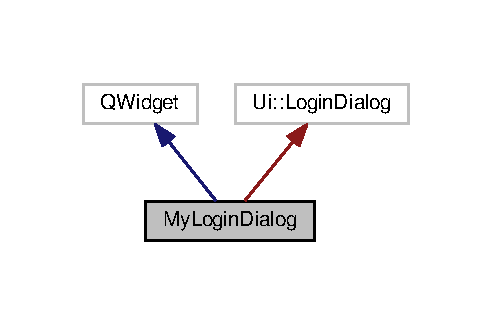
\includegraphics[width=236pt]{d5/d81/classMyLoginDialog__inherit__graph}
\end{center}
\end{figure}


Collaboration diagram for My\+Login\+Dialog\+:
\nopagebreak
\begin{figure}[H]
\begin{center}
\leavevmode
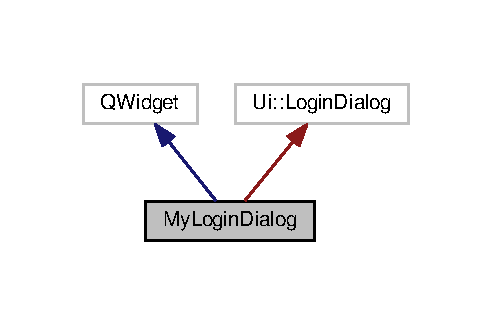
\includegraphics[width=236pt]{db/d47/classMyLoginDialog__coll__graph}
\end{center}
\end{figure}
\subsection*{Public Slots}
\begin{DoxyCompactItemize}
\item 
void \hyperlink{classMyLoginDialog_ab850edc55bc360a5271f8da572d9b84b}{on\+\_\+login\+\_\+button\+\_\+clicked} (void)
\begin{DoxyCompactList}\small\item\em Slot chamado para realizar a operação de login. \end{DoxyCompactList}\item 
void \hyperlink{classMyLoginDialog_a98b534e1f3e50217b7d0d603846f6fa3}{on\+\_\+cancel\+\_\+button\+\_\+clicked} (void)
\begin{DoxyCompactList}\small\item\em Slot chamado para finalizar a aplicação. \end{DoxyCompactList}\item 
void \hyperlink{classMyLoginDialog_a6def7158f19720b26ac23274b38ddc2d}{read\+Message} (Q\+Json\+Object json\+Object)
\begin{DoxyCompactList}\small\item\em Slot chamado quando o socket recebe uma mensagem de resposta do servidor. \end{DoxyCompactList}\end{DoxyCompactItemize}
\subsection*{Signals}
\begin{DoxyCompactItemize}
\item 
void \hyperlink{classMyLoginDialog_af34aa4fb816da6adb7813ced2779cc3e}{logged} (Q\+String username, bool admin\+Level)
\begin{DoxyCompactList}\small\item\em Signal emitido quando a operação de login é realizada com sucesso. \end{DoxyCompactList}\item 
void \hyperlink{classMyLoginDialog_a81b2fde13842c6557400e0e35b9dd1e0}{quit} (void)\hypertarget{classMyLoginDialog_a81b2fde13842c6557400e0e35b9dd1e0}{}\label{classMyLoginDialog_a81b2fde13842c6557400e0e35b9dd1e0}

\begin{DoxyCompactList}\small\item\em Signal emitido para finalizar a aplicação. \end{DoxyCompactList}\end{DoxyCompactItemize}
\subsection*{Public Member Functions}
\begin{DoxyCompactItemize}
\item 
\hyperlink{classMyLoginDialog_ae20170dfe9e23fc1b794d3b5a2d2cc97}{My\+Login\+Dialog} (Q\+Widget $\ast$parent=nullptr)
\begin{DoxyCompactList}\small\item\em Construtor Padrão para a classe \hyperlink{classMyLoginDialog}{My\+Login\+Dialog}. \end{DoxyCompactList}\end{DoxyCompactItemize}
\subsection*{Private Attributes}
\begin{DoxyCompactItemize}
\item 
Q\+Tcp\+Socket \hyperlink{classMyLoginDialog_aea07f561f3a3e17b6596da377a538e4f}{tcp\+Socket}\hypertarget{classMyLoginDialog_aea07f561f3a3e17b6596da377a538e4f}{}\label{classMyLoginDialog_aea07f561f3a3e17b6596da377a538e4f}

\begin{DoxyCompactList}\small\item\em T\+C\+P\+Socket utilizado pela aplicação para comunicar com servidor. \end{DoxyCompactList}\end{DoxyCompactItemize}
\subsection*{Friends}
\begin{DoxyCompactItemize}
\item 
class \hyperlink{classMyLoginDialog_aec613ce0d143a48322f72a2b90819fcb}{My\+Login\+Dialog\+Test}\hypertarget{classMyLoginDialog_aec613ce0d143a48322f72a2b90819fcb}{}\label{classMyLoginDialog_aec613ce0d143a48322f72a2b90819fcb}

\begin{DoxyCompactList}\small\item\em Classe para Testes de \hyperlink{classMyLoginDialog}{My\+Login\+Dialog}. \end{DoxyCompactList}\end{DoxyCompactItemize}


\subsection{Detailed Description}
Classe para gerenciar as requisições de login. 

Esta classe gerencia as iterações do usuário com uma janela de login e realiza a validação dos dados em um servidor. 

\subsection{Constructor \& Destructor Documentation}
\index{My\+Login\+Dialog@{My\+Login\+Dialog}!My\+Login\+Dialog@{My\+Login\+Dialog}}
\index{My\+Login\+Dialog@{My\+Login\+Dialog}!My\+Login\+Dialog@{My\+Login\+Dialog}}
\subsubsection[{\texorpdfstring{My\+Login\+Dialog(\+Q\+Widget $\ast$parent=nullptr)}{MyLoginDialog(QWidget *parent=nullptr)}}]{\setlength{\rightskip}{0pt plus 5cm}My\+Login\+Dialog\+::\+My\+Login\+Dialog (
\begin{DoxyParamCaption}
\item[{Q\+Widget $\ast$}]{parent = {\ttfamily nullptr}}
\end{DoxyParamCaption}
)}\hypertarget{classMyLoginDialog_ae20170dfe9e23fc1b794d3b5a2d2cc97}{}\label{classMyLoginDialog_ae20170dfe9e23fc1b794d3b5a2d2cc97}


Construtor Padrão para a classe \hyperlink{classMyLoginDialog}{My\+Login\+Dialog}. 

Inicializa o atributo parent, configura a interface por meio do método \textquotesingle{}setup\+Ui\textquotesingle{} da classe pai Login\+Dialog e conecta o slot para a leitura de mensagens do servidor.


\begin{DoxyParams}{Parameters}
{\em parent} & Referência ao componente pai. \\
\hline
\end{DoxyParams}


\subsection{Member Function Documentation}
\index{My\+Login\+Dialog@{My\+Login\+Dialog}!logged@{logged}}
\index{logged@{logged}!My\+Login\+Dialog@{My\+Login\+Dialog}}
\subsubsection[{\texorpdfstring{logged}{logged}}]{\setlength{\rightskip}{0pt plus 5cm}void My\+Login\+Dialog\+::logged (
\begin{DoxyParamCaption}
\item[{Q\+String}]{username, }
\item[{bool}]{admin\+Level}
\end{DoxyParamCaption}
)\hspace{0.3cm}{\ttfamily [signal]}}\hypertarget{classMyLoginDialog_af34aa4fb816da6adb7813ced2779cc3e}{}\label{classMyLoginDialog_af34aa4fb816da6adb7813ced2779cc3e}


Signal emitido quando a operação de login é realizada com sucesso. 


\begin{DoxyParams}{Parameters}
{\em username} & Nome do usuário. \\
\hline
{\em admin\+Level} & Flag identificando se o usuário é administrador. \\
\hline
\end{DoxyParams}
\index{My\+Login\+Dialog@{My\+Login\+Dialog}!on\+\_\+cancel\+\_\+button\+\_\+clicked@{on\+\_\+cancel\+\_\+button\+\_\+clicked}}
\index{on\+\_\+cancel\+\_\+button\+\_\+clicked@{on\+\_\+cancel\+\_\+button\+\_\+clicked}!My\+Login\+Dialog@{My\+Login\+Dialog}}
\subsubsection[{\texorpdfstring{on\+\_\+cancel\+\_\+button\+\_\+clicked}{on_cancel_button_clicked}}]{\setlength{\rightskip}{0pt plus 5cm}void My\+Login\+Dialog\+::on\+\_\+cancel\+\_\+button\+\_\+clicked (
\begin{DoxyParamCaption}
\item[{void}]{}
\end{DoxyParamCaption}
)\hspace{0.3cm}{\ttfamily [slot]}}\hypertarget{classMyLoginDialog_a98b534e1f3e50217b7d0d603846f6fa3}{}\label{classMyLoginDialog_a98b534e1f3e50217b7d0d603846f6fa3}


Slot chamado para finalizar a aplicação. 

\begin{DoxySeeAlso}{See also}
\hyperlink{classMyLoginDialog_a81b2fde13842c6557400e0e35b9dd1e0}{My\+Login\+Dialog\+::quit()}. 
\end{DoxySeeAlso}
\index{My\+Login\+Dialog@{My\+Login\+Dialog}!on\+\_\+login\+\_\+button\+\_\+clicked@{on\+\_\+login\+\_\+button\+\_\+clicked}}
\index{on\+\_\+login\+\_\+button\+\_\+clicked@{on\+\_\+login\+\_\+button\+\_\+clicked}!My\+Login\+Dialog@{My\+Login\+Dialog}}
\subsubsection[{\texorpdfstring{on\+\_\+login\+\_\+button\+\_\+clicked}{on_login_button_clicked}}]{\setlength{\rightskip}{0pt plus 5cm}void My\+Login\+Dialog\+::on\+\_\+login\+\_\+button\+\_\+clicked (
\begin{DoxyParamCaption}
\item[{void}]{}
\end{DoxyParamCaption}
)\hspace{0.3cm}{\ttfamily [slot]}}\hypertarget{classMyLoginDialog_ab850edc55bc360a5271f8da572d9b84b}{}\label{classMyLoginDialog_ab850edc55bc360a5271f8da572d9b84b}


Slot chamado para realizar a operação de login. 

Recupera as informações da interface e realiza um requisição de autenticação ao servidor.

\begin{DoxySeeAlso}{See also}
\hyperlink{classMyLoginDialog_a6def7158f19720b26ac23274b38ddc2d}{My\+Login\+Dialog\+::read\+Message()}. 
\end{DoxySeeAlso}
\index{My\+Login\+Dialog@{My\+Login\+Dialog}!read\+Message@{read\+Message}}
\index{read\+Message@{read\+Message}!My\+Login\+Dialog@{My\+Login\+Dialog}}
\subsubsection[{\texorpdfstring{read\+Message}{readMessage}}]{\setlength{\rightskip}{0pt plus 5cm}void My\+Login\+Dialog\+::read\+Message (
\begin{DoxyParamCaption}
\item[{Q\+Json\+Object}]{json\+Object}
\end{DoxyParamCaption}
)\hspace{0.3cm}{\ttfamily [slot]}}\hypertarget{classMyLoginDialog_a6def7158f19720b26ac23274b38ddc2d}{}\label{classMyLoginDialog_a6def7158f19720b26ac23274b38ddc2d}


Slot chamado quando o socket recebe uma mensagem de resposta do servidor. 

Esse método recebe uma resposta do servidor sobre a tentativa de login. Caso positivo emite um signal informando que o usuário foi autenticado. Caso contrário mostra uma janela de erro.

\begin{DoxySeeAlso}{See also}
\hyperlink{classMyLoginDialog_ab850edc55bc360a5271f8da572d9b84b}{My\+Login\+Dialog\+::on\+\_\+login\+\_\+button\+\_\+clicked()}, My\+Login\+Dialog\+::logged(\+Q\+String,bool,\+Q\+String,int). 
\end{DoxySeeAlso}


The documentation for this class was generated from the following files\+:\begin{DoxyCompactItemize}
\item 
Calc\+Client/src/gui/\hyperlink{mylogindialog_8h}{mylogindialog.\+h}\item 
Calc\+Client/src/gui/\hyperlink{mylogindialog_8cpp}{mylogindialog.\+cpp}\end{DoxyCompactItemize}

\hypertarget{classServer}{}\section{Server Class Reference}
\label{classServer}\index{Server@{Server}}


Clase para gerenciamento de servidor T\+CP.  




{\ttfamily \#include $<$server.\+h$>$}



Inheritance diagram for Server\+:\nopagebreak
\begin{figure}[H]
\begin{center}
\leavevmode
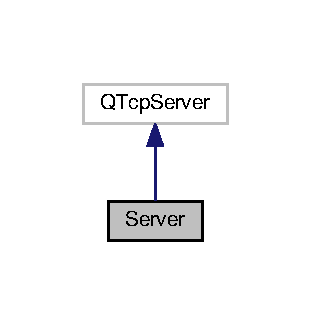
\includegraphics[width=149pt]{d3/dd7/classServer__inherit__graph}
\end{center}
\end{figure}


Collaboration diagram for Server\+:\nopagebreak
\begin{figure}[H]
\begin{center}
\leavevmode
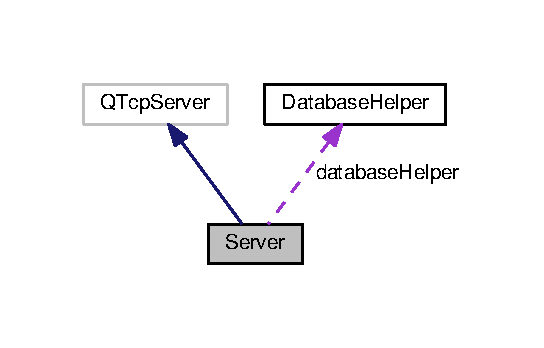
\includegraphics[width=149pt]{de/ddc/classServer__coll__graph}
\end{center}
\end{figure}
\subsection*{Protected Member Functions}
\begin{DoxyCompactItemize}
\item 
virtual void \hyperlink{classServer_a2397527620515d7e18fc599b22fb64ae}{incoming\+Connection} (qintptr socket\+Descriptor)=0
\begin{DoxyCompactList}\small\item\em Método para delegar o tratamento de uma conexão a uma thread trabalhadora auxiliar. \end{DoxyCompactList}\end{DoxyCompactItemize}


\subsection{Detailed Description}
Clase para gerenciamento de servidor T\+CP. 

\subsection{Member Function Documentation}
\index{Server@{Server}!incoming\+Connection@{incoming\+Connection}}
\index{incoming\+Connection@{incoming\+Connection}!Server@{Server}}
\subsubsection[{\texorpdfstring{incoming\+Connection(qintptr socket\+Descriptor)=0}{incomingConnection(qintptr socketDescriptor)=0}}]{\setlength{\rightskip}{0pt plus 5cm}virtual void Server\+::incoming\+Connection (
\begin{DoxyParamCaption}
\item[{qintptr}]{socket\+Descriptor}
\end{DoxyParamCaption}
)\hspace{0.3cm}{\ttfamily [protected]}, {\ttfamily [pure virtual]}}\hypertarget{classServer_a2397527620515d7e18fc599b22fb64ae}{}\label{classServer_a2397527620515d7e18fc599b22fb64ae}


Método para delegar o tratamento de uma conexão a uma thread trabalhadora auxiliar. 

Ao receber uma conexão o servidor delega o tratamento dela a um thread auxiliar e volta a escutar as transmissões.


\begin{DoxyParams}{Parameters}
{\em socket\+Descriptor} & Informações de configuração do socket.\\
\hline
\end{DoxyParams}
\begin{DoxySeeAlso}{See also}
\hyperlink{classWorkerThread}{Worker\+Thread}. 
\end{DoxySeeAlso}


Implemented in \hyperlink{classServerImpl_a54dda38486e9964432b501f7da00ed97}{Server\+Impl}.



The documentation for this class was generated from the following file\+:\begin{DoxyCompactItemize}
\item 
Calc\+Server/\hyperlink{server_8h}{server.\+h}\end{DoxyCompactItemize}

\hypertarget{classWorkerThread}{}\section{Worker\+Thread Class Reference}
\label{classWorkerThread}\index{Worker\+Thread@{Worker\+Thread}}


Interface para thread de trabalho auxiliar.  




{\ttfamily \#include $<$workerthread.\+h$>$}



Inheritance diagram for Worker\+Thread\+:\nopagebreak
\begin{figure}[H]
\begin{center}
\leavevmode
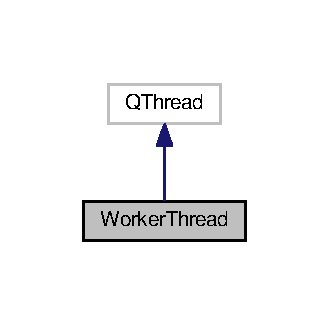
\includegraphics[width=177pt]{d3/da8/classWorkerThread__inherit__graph}
\end{center}
\end{figure}
\subsection*{Public Member Functions}
\begin{DoxyCompactItemize}
\item 
virtual void \hyperlink{classWorkerThread_a008dd6f762a2c20641afbb2a69319ca4}{run} ()=0
\begin{DoxyCompactList}\small\item\em Método para delegação do tratamento de uma mensagem recebida e envio da respostas. \end{DoxyCompactList}\item 
virtual void \hyperlink{classWorkerThread_a4d6d532dfbb27c5a435018ea697acb11}{start} ()=0\hypertarget{classWorkerThread_a4d6d532dfbb27c5a435018ea697acb11}{}\label{classWorkerThread_a4d6d532dfbb27c5a435018ea697acb11}

\begin{DoxyCompactList}\small\item\em Método para o inicio de execução de uma \hyperlink{classWorkerThread}{Worker\+Thread}. \end{DoxyCompactList}\item 
virtual void \hyperlink{classWorkerThread_a270d44343c31516acebd9544788e3886}{finished} ()=0\hypertarget{classWorkerThread_a270d44343c31516acebd9544788e3886}{}\label{classWorkerThread_a270d44343c31516acebd9544788e3886}

\begin{DoxyCompactList}\small\item\em Representa o fim de execução de \hyperlink{classWorkerThread}{Worker\+Thread}. \end{DoxyCompactList}\item 
virtual void \hyperlink{classWorkerThread_abf55cfb94dd10a2a3b2ff3896473c11b}{delete\+Later} ()=0\hypertarget{classWorkerThread_abf55cfb94dd10a2a3b2ff3896473c11b}{}\label{classWorkerThread_abf55cfb94dd10a2a3b2ff3896473c11b}

\begin{DoxyCompactList}\small\item\em Responsavel por desalocar elementos da \hyperlink{classWorkerThread}{Worker\+Thread}. \end{DoxyCompactList}\item 
virtual Q\+Object $\ast$ \hyperlink{classWorkerThread_a7cce841d4e0b98ebdeb0c7027045dfc4}{get\+Q\+Object} ()=0
\begin{DoxyCompactList}\small\item\em Método retorna uma referência a um objeto Q\+Object correspondente a essa classe. \end{DoxyCompactList}\end{DoxyCompactItemize}


\subsection{Detailed Description}
Interface para thread de trabalho auxiliar. 

\subsection{Member Function Documentation}
\index{Worker\+Thread@{Worker\+Thread}!get\+Q\+Object@{get\+Q\+Object}}
\index{get\+Q\+Object@{get\+Q\+Object}!Worker\+Thread@{Worker\+Thread}}
\subsubsection[{\texorpdfstring{get\+Q\+Object()=0}{getQObject()=0}}]{\setlength{\rightskip}{0pt plus 5cm}virtual Q\+Object$\ast$ Worker\+Thread\+::get\+Q\+Object (
\begin{DoxyParamCaption}
{}
\end{DoxyParamCaption}
)\hspace{0.3cm}{\ttfamily [pure virtual]}}\hypertarget{classWorkerThread_a7cce841d4e0b98ebdeb0c7027045dfc4}{}\label{classWorkerThread_a7cce841d4e0b98ebdeb0c7027045dfc4}


Método retorna uma referência a um objeto Q\+Object correspondente a essa classe. 

\begin{DoxyReturn}{Returns}
Referencia ao Q\+Object correspondente a classe. 
\end{DoxyReturn}


Implemented in \hyperlink{classWorkerThreadImpl_a30689eaffcb664bc95644bf497ea1446}{Worker\+Thread\+Impl}.

\index{Worker\+Thread@{Worker\+Thread}!run@{run}}
\index{run@{run}!Worker\+Thread@{Worker\+Thread}}
\subsubsection[{\texorpdfstring{run()=0}{run()=0}}]{\setlength{\rightskip}{0pt plus 5cm}virtual void Worker\+Thread\+::run (
\begin{DoxyParamCaption}
{}
\end{DoxyParamCaption}
)\hspace{0.3cm}{\ttfamily [pure virtual]}}\hypertarget{classWorkerThread_a008dd6f762a2c20641afbb2a69319ca4}{}\label{classWorkerThread_a008dd6f762a2c20641afbb2a69319ca4}


Método para delegação do tratamento de uma mensagem recebida e envio da respostas. 

Este método recebe um byte array correspondente a um objeto J\+S\+ON, após isso cria um objeto J\+S\+ON e delega a resolução da mensagem para o método handl\+Message. Por fim, recebe a resposta da mensagem, codifica ela e envia ao cliente pela rede.

\begin{DoxySeeAlso}{See also}
\hyperlink{classWorkerThreadImpl_ac1ced60fd043f7dca8a7e7e1857a91cb}{Worker\+Thread\+Impl\+::handle\+Message(\+Q\+Json\+Object)}, \hyperlink{classWorkerThreadImpl_ae260562530b71dc55a6d360d5e4d896d}{Worker\+Thread\+Impl\+::error(\+Q\+Tcp\+Socket\+::\+Socket\+Error)}. 
\end{DoxySeeAlso}


Implemented in \hyperlink{classWorkerThreadImpl_a24ef315ed0b7914ffd099c23a5a6e16c}{Worker\+Thread\+Impl}.



The documentation for this class was generated from the following file\+:\begin{DoxyCompactItemize}
\item 
Calc\+Server/\hyperlink{workerthread_8h}{workerthread.\+h}\end{DoxyCompactItemize}

\chapter{File Documentation}
\hypertarget{mycalcwindow_8cpp}{}\section{Calc\+Client/mycalcwindow.cpp File Reference}
\label{mycalcwindow_8cpp}\index{Calc\+Client/mycalcwindow.\+cpp@{Calc\+Client/mycalcwindow.\+cpp}}
{\ttfamily \#include $<$Q\+Sql\+Query$>$}\\*
{\ttfamily \#include $<$Q\+Message\+Box$>$}\\*
{\ttfamily \#include $<$Q\+Debug$>$}\\*
{\ttfamily \#include $<$Q\+Sql\+Error$>$}\\*
{\ttfamily \#include $<$Q\+Json\+Object$>$}\\*
{\ttfamily \#include $<$Q\+Json\+Document$>$}\\*
{\ttfamily \#include $<$string$>$}\\*
{\ttfamily \#include $<$sstream$>$}\\*
{\ttfamily \#include $<$iostream$>$}\\*
{\ttfamily \#include \char`\"{}mycalcwindow.\+h\char`\"{}}\\*
{\ttfamily \#include \char`\"{}ui\+\_\+calcwindow.\+h\char`\"{}}\\*
Include dependency graph for mycalcwindow.\+cpp\+:\nopagebreak
\begin{figure}[H]
\begin{center}
\leavevmode
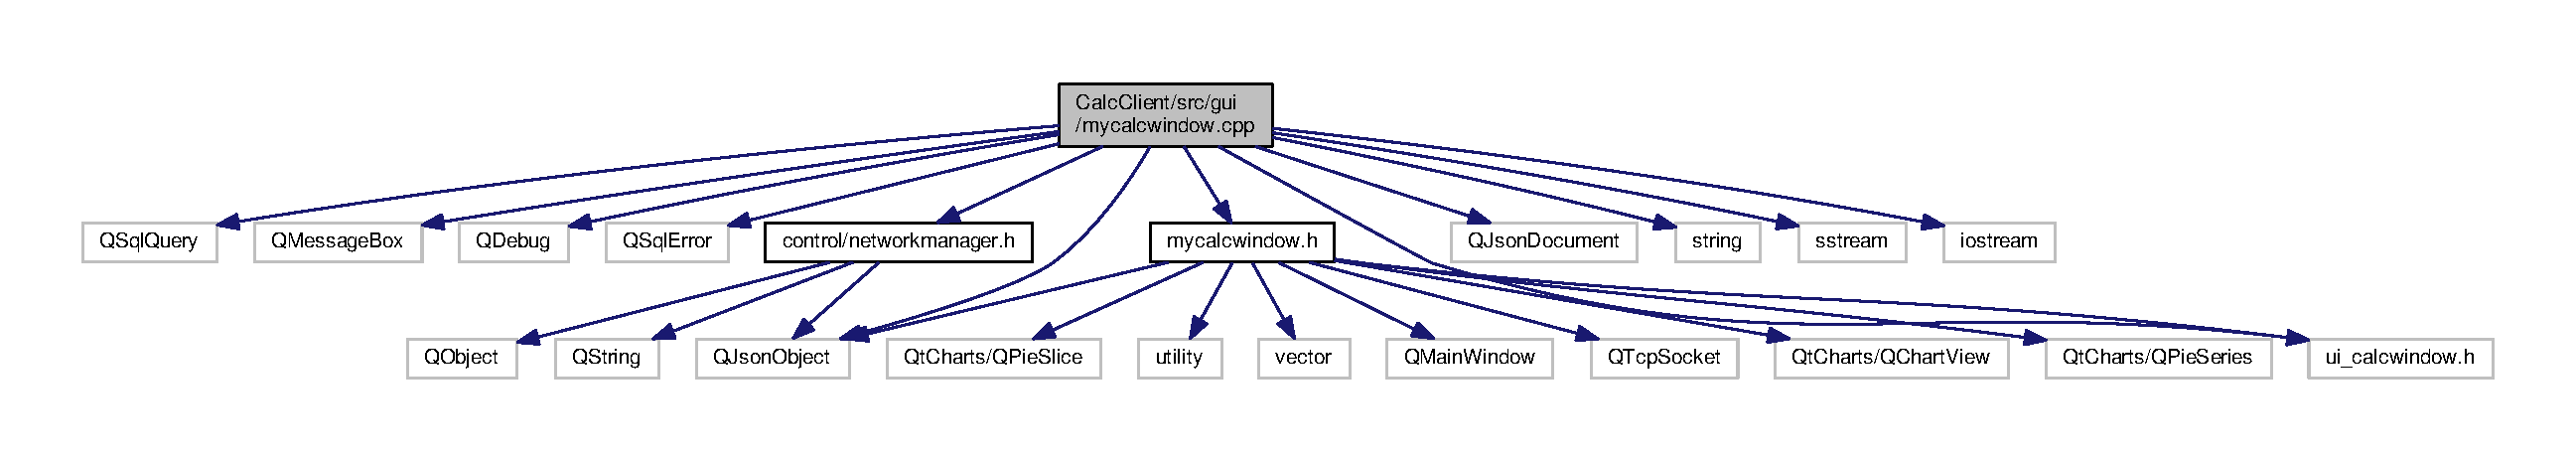
\includegraphics[width=350pt]{d1/d12/mycalcwindow_8cpp__incl}
\end{center}
\end{figure}
\subsection*{Macros}
\begin{DoxyCompactItemize}
\item 
\#define \hyperlink{mycalcwindow_8cpp_ad72dbcf6d0153db1b8d8a58001feed83}{D\+E\+B\+UG}
\end{DoxyCompactItemize}


\subsection{Detailed Description}
Arquivo contendo a implementação da Classe \hyperlink{classMyCalcWindow}{My\+Calc\+Window}. 

\subsection{Macro Definition Documentation}
\index{mycalcwindow.\+cpp@{mycalcwindow.\+cpp}!D\+E\+B\+UG@{D\+E\+B\+UG}}
\index{D\+E\+B\+UG@{D\+E\+B\+UG}!mycalcwindow.\+cpp@{mycalcwindow.\+cpp}}
\subsubsection[{\texorpdfstring{D\+E\+B\+UG}{DEBUG}}]{\setlength{\rightskip}{0pt plus 5cm}\#define D\+E\+B\+UG}\hypertarget{mycalcwindow_8cpp_ad72dbcf6d0153db1b8d8a58001feed83}{}\label{mycalcwindow_8cpp_ad72dbcf6d0153db1b8d8a58001feed83}
Flag demarcando se as mensagens de debug devem ou não serem exibidas. 
\hypertarget{mycalcwindow_8h}{}\section{Calc\+Client/src/gui/mycalcwindow.h File Reference}
\label{mycalcwindow_8h}\index{Calc\+Client/src/gui/mycalcwindow.\+h@{Calc\+Client/src/gui/mycalcwindow.\+h}}
{\ttfamily \#include $<$Q\+Main\+Window$>$}\\*
{\ttfamily \#include $<$Q\+Tcp\+Socket$>$}\\*
{\ttfamily \#include $<$Qt\+Charts/\+Q\+Chart\+View$>$}\\*
{\ttfamily \#include $<$Qt\+Charts/\+Q\+Pie\+Series$>$}\\*
{\ttfamily \#include $<$Qt\+Charts/\+Q\+Pie\+Slice$>$}\\*
{\ttfamily \#include $<$Q\+Json\+Object$>$}\\*
{\ttfamily \#include $<$utility$>$}\\*
{\ttfamily \#include $<$vector$>$}\\*
{\ttfamily \#include \char`\"{}ui\+\_\+calcwindow.\+h\char`\"{}}\\*
Include dependency graph for mycalcwindow.\+h\+:
\nopagebreak
\begin{figure}[H]
\begin{center}
\leavevmode
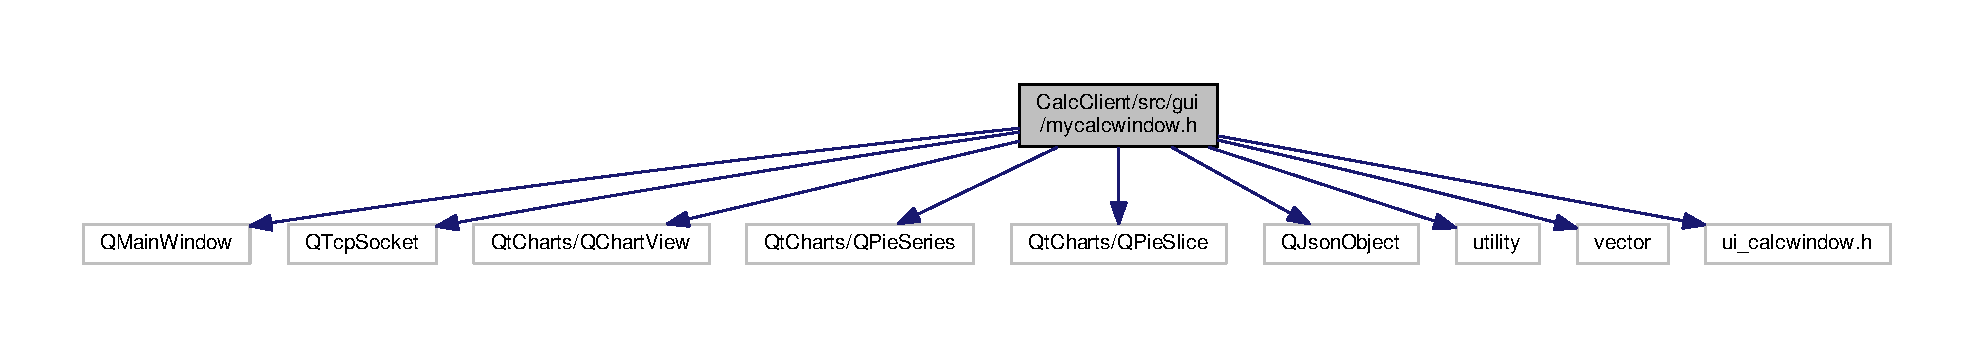
\includegraphics[width=350pt]{d0/d90/mycalcwindow_8h__incl}
\end{center}
\end{figure}
This graph shows which files directly or indirectly include this file\+:
\nopagebreak
\begin{figure}[H]
\begin{center}
\leavevmode
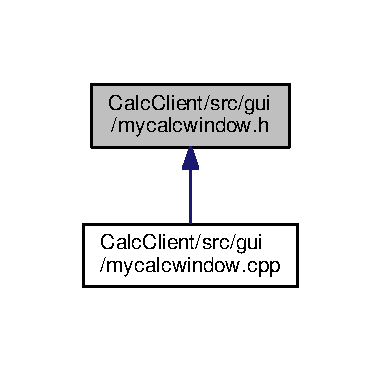
\includegraphics[width=183pt]{d1/d82/mycalcwindow_8h__dep__incl}
\end{center}
\end{figure}
\subsection*{Classes}
\begin{DoxyCompactItemize}
\item 
class \hyperlink{classMyCalcWindow}{My\+Calc\+Window}
\begin{DoxyCompactList}\small\item\em Classe para gerenciar as ações de uma calculadora. \end{DoxyCompactList}\end{DoxyCompactItemize}


\subsection{Detailed Description}
Arquivo contendo a declaração da Classe \hyperlink{classMyCalcWindow}{My\+Calc\+Window}. 
\hypertarget{mylogindialog_8cpp}{}\section{Calc\+Client/mylogindialog.cpp File Reference}
\label{mylogindialog_8cpp}\index{Calc\+Client/mylogindialog.\+cpp@{Calc\+Client/mylogindialog.\+cpp}}
{\ttfamily \#include \char`\"{}mylogindialog.\+h\char`\"{}}\\*
{\ttfamily \#include \char`\"{}ui\+\_\+logindialog.\+h\char`\"{}}\\*
{\ttfamily \#include $<$Q\+Message\+Box$>$}\\*
{\ttfamily \#include $<$Q\+String$>$}\\*
{\ttfamily \#include $<$Q\+Sql\+Database$>$}\\*
{\ttfamily \#include $<$Q\+Sql\+Query$>$}\\*
{\ttfamily \#include $<$Q\+Dialog$>$}\\*
{\ttfamily \#include $<$Q\+Debug$>$}\\*
{\ttfamily \#include $<$Q\+Json\+Object$>$}\\*
{\ttfamily \#include $<$Q\+Json\+Document$>$}\\*
{\ttfamily \#include $<$iostream$>$}\\*
Include dependency graph for mylogindialog.\+cpp\+:\nopagebreak
\begin{figure}[H]
\begin{center}
\leavevmode
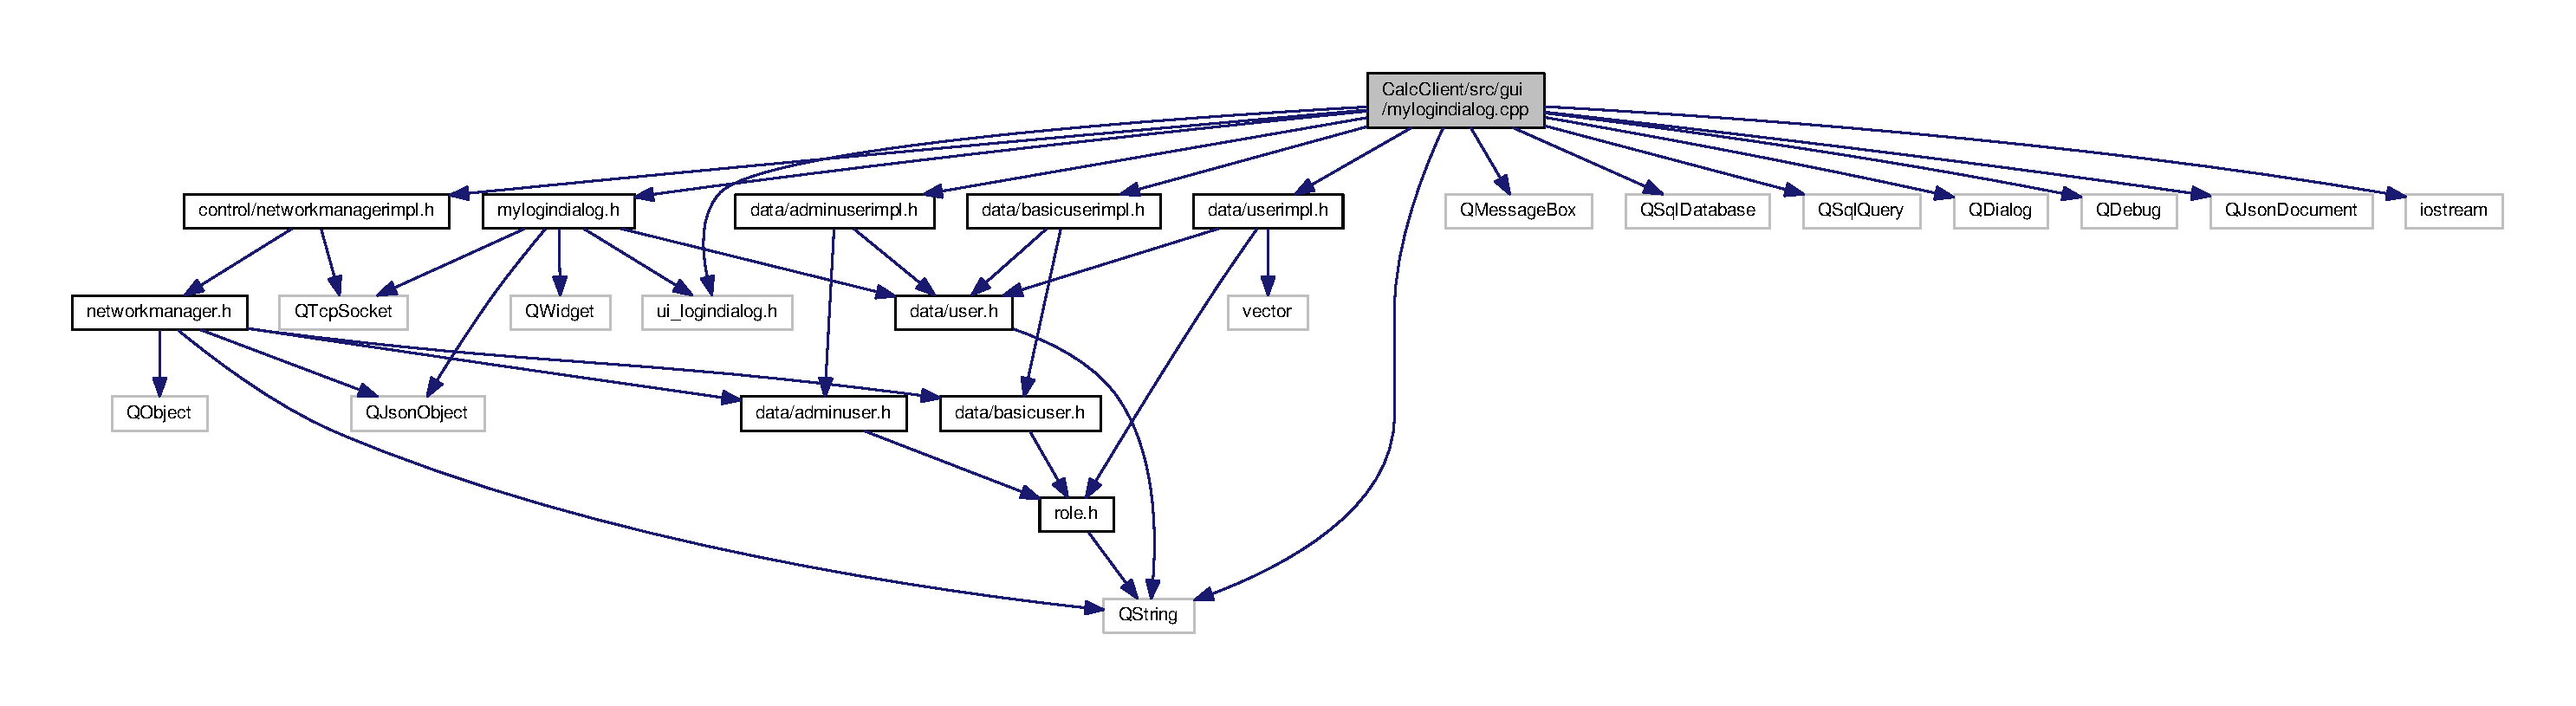
\includegraphics[width=350pt]{d4/d68/mylogindialog_8cpp__incl}
\end{center}
\end{figure}
\subsection*{Macros}
\begin{DoxyCompactItemize}
\item 
\#define \hyperlink{mylogindialog_8cpp_ad72dbcf6d0153db1b8d8a58001feed83}{D\+E\+B\+UG}
\end{DoxyCompactItemize}


\subsection{Detailed Description}
Arquivo contendo a implementação da Classe \hyperlink{classMyLoginDialog}{My\+Login\+Dialog}. 

\subsection{Macro Definition Documentation}
\index{mylogindialog.\+cpp@{mylogindialog.\+cpp}!D\+E\+B\+UG@{D\+E\+B\+UG}}
\index{D\+E\+B\+UG@{D\+E\+B\+UG}!mylogindialog.\+cpp@{mylogindialog.\+cpp}}
\subsubsection[{\texorpdfstring{D\+E\+B\+UG}{DEBUG}}]{\setlength{\rightskip}{0pt plus 5cm}\#define D\+E\+B\+UG}\hypertarget{mylogindialog_8cpp_ad72dbcf6d0153db1b8d8a58001feed83}{}\label{mylogindialog_8cpp_ad72dbcf6d0153db1b8d8a58001feed83}
Flag demarcando se as mensagens de debug devem ou não serem exibidas. 
\hypertarget{mylogindialog_8h}{}\section{Calc\+Client/src/gui/mylogindialog.h File Reference}
\label{mylogindialog_8h}\index{Calc\+Client/src/gui/mylogindialog.\+h@{Calc\+Client/src/gui/mylogindialog.\+h}}
{\ttfamily \#include $<$Q\+Widget$>$}\\*
{\ttfamily \#include $<$Q\+Tcp\+Socket$>$}\\*
{\ttfamily \#include $<$Q\+Json\+Object$>$}\\*
{\ttfamily \#include \char`\"{}ui\+\_\+logindialog.\+h\char`\"{}}\\*
Include dependency graph for mylogindialog.\+h\+:
\nopagebreak
\begin{figure}[H]
\begin{center}
\leavevmode
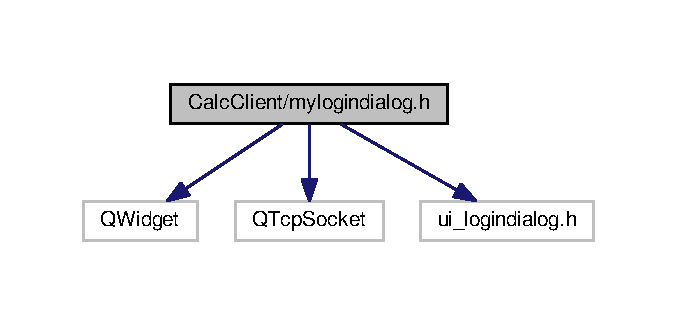
\includegraphics[width=350pt]{d8/d9e/mylogindialog_8h__incl}
\end{center}
\end{figure}
This graph shows which files directly or indirectly include this file\+:
\nopagebreak
\begin{figure}[H]
\begin{center}
\leavevmode
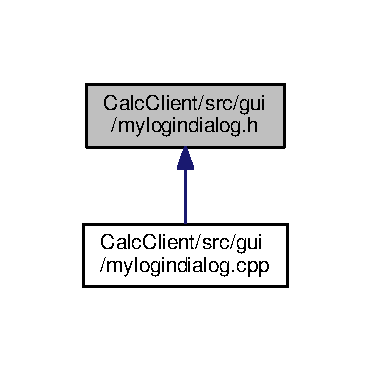
\includegraphics[width=178pt]{d7/d40/mylogindialog_8h__dep__incl}
\end{center}
\end{figure}
\subsection*{Classes}
\begin{DoxyCompactItemize}
\item 
class \hyperlink{classMyLoginDialog}{My\+Login\+Dialog}
\begin{DoxyCompactList}\small\item\em Classe para gerenciar as requisições de login. \end{DoxyCompactList}\end{DoxyCompactItemize}


\subsection{Detailed Description}
Arquivo contendo a declaração da Classe \hyperlink{classMyLoginDialog}{My\+Login\+Dialog}. 
\hypertarget{databasehelper_8h}{}\section{Calc\+Server/src/database/databasehelper.h File Reference}
\label{databasehelper_8h}\index{Calc\+Server/src/database/databasehelper.\+h@{Calc\+Server/src/database/databasehelper.\+h}}
{\ttfamily \#include $<$Q\+String$>$}\\*
{\ttfamily \#include $<$utility$>$}\\*
{\ttfamily \#include $<$vector$>$}\\*
Include dependency graph for databasehelper.\+h\+:
\nopagebreak
\begin{figure}[H]
\begin{center}
\leavevmode
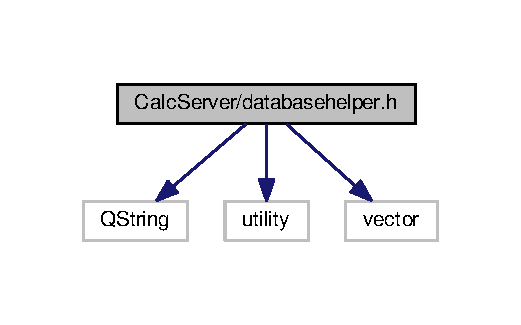
\includegraphics[width=250pt]{da/dea/databasehelper_8h__incl}
\end{center}
\end{figure}
This graph shows which files directly or indirectly include this file\+:
\nopagebreak
\begin{figure}[H]
\begin{center}
\leavevmode
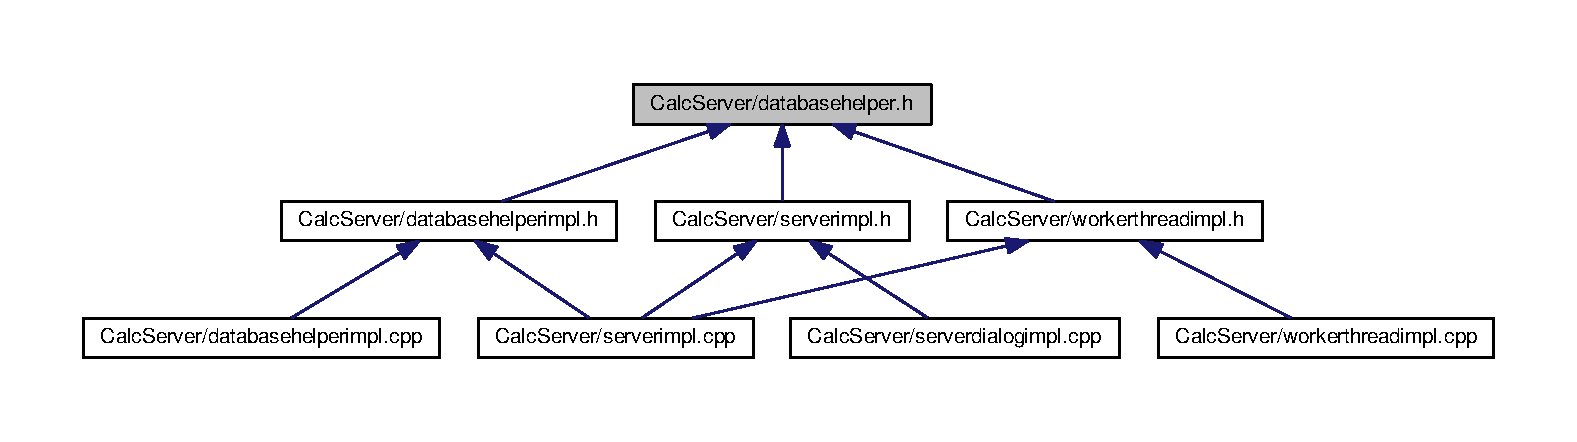
\includegraphics[width=350pt]{d2/d71/databasehelper_8h__dep__incl}
\end{center}
\end{figure}
\subsection*{Classes}
\begin{DoxyCompactItemize}
\item 
class \hyperlink{classDatabaseHelper}{Database\+Helper}
\begin{DoxyCompactList}\small\item\em Interface para acesso a um banco de dados. \end{DoxyCompactList}\end{DoxyCompactItemize}


\subsection{Detailed Description}
Arquivo contendo a declaração da Interface \hyperlink{classDatabaseHelper}{Database\+Helper}. 
\hypertarget{databasehelperimpl_8cpp}{}\section{Calc\+Server/databasehelperimpl.cpp File Reference}
\label{databasehelperimpl_8cpp}\index{Calc\+Server/databasehelperimpl.\+cpp@{Calc\+Server/databasehelperimpl.\+cpp}}
{\ttfamily \#include \char`\"{}databasehelperimpl.\+h\char`\"{}}\\*
{\ttfamily \#include $<$Q\+Sql\+Query$>$}\\*
{\ttfamily \#include $<$Q\+Variant$>$}\\*
Include dependency graph for databasehelperimpl.\+cpp\+:\nopagebreak
\begin{figure}[H]
\begin{center}
\leavevmode
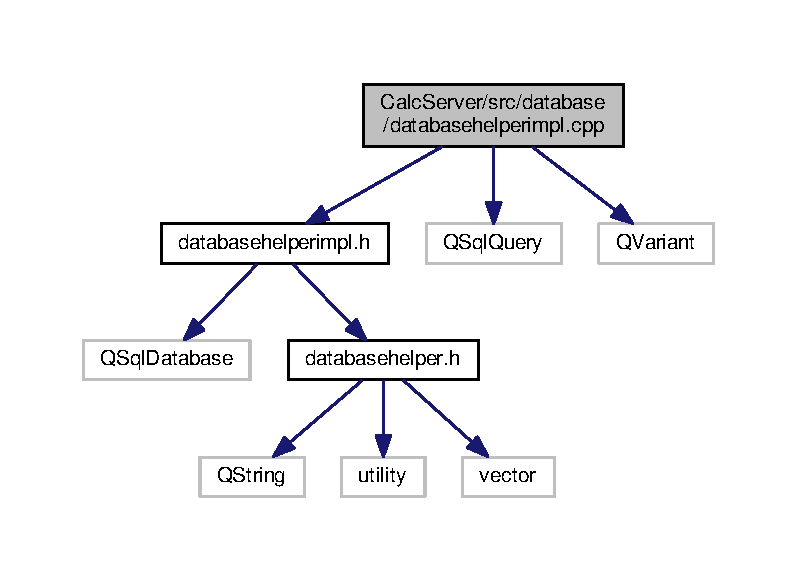
\includegraphics[width=350pt]{d7/d6c/databasehelperimpl_8cpp__incl}
\end{center}
\end{figure}


\subsection{Detailed Description}
Arquivo contendo a implementação da Classe \hyperlink{classDatabaseHelperImpl}{Database\+Helper\+Impl}. 
\hypertarget{databasehelperimpl_8h}{}\section{Calc\+Server/databasehelperimpl.h File Reference}
\label{databasehelperimpl_8h}\index{Calc\+Server/databasehelperimpl.\+h@{Calc\+Server/databasehelperimpl.\+h}}
{\ttfamily \#include $<$Q\+Sql\+Database$>$}\\*
{\ttfamily \#include \char`\"{}databasehelper.\+h\char`\"{}}\\*
Include dependency graph for databasehelperimpl.\+h\+:\nopagebreak
\begin{figure}[H]
\begin{center}
\leavevmode
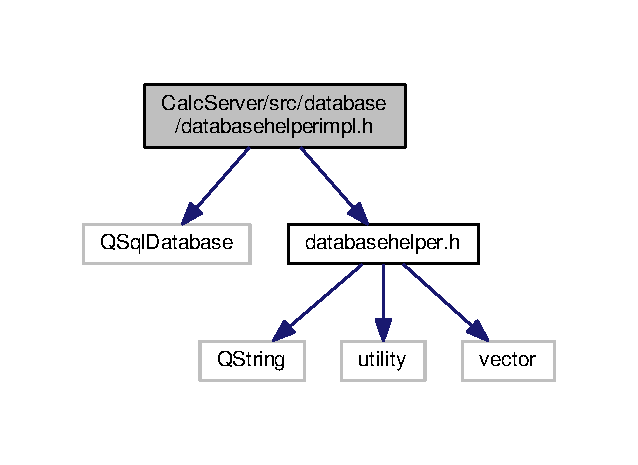
\includegraphics[width=306pt]{d8/d9e/databasehelperimpl_8h__incl}
\end{center}
\end{figure}
This graph shows which files directly or indirectly include this file\+:\nopagebreak
\begin{figure}[H]
\begin{center}
\leavevmode
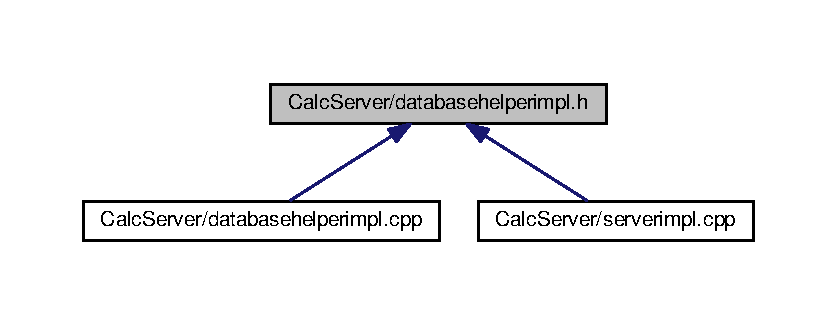
\includegraphics[width=350pt]{d3/d1f/databasehelperimpl_8h__dep__incl}
\end{center}
\end{figure}
\subsection*{Classes}
\begin{DoxyCompactItemize}
\item 
class \hyperlink{classDatabaseHelperImpl}{Database\+Helper\+Impl}
\begin{DoxyCompactList}\small\item\em Implementação da Interface \hyperlink{classDatabaseHelper}{Database\+Helper} para acesso ao banco de dados S\+Q\+Lite. \end{DoxyCompactList}\end{DoxyCompactItemize}


\subsection{Detailed Description}
Arquivo contendo a declaração da Classe \hyperlink{classDatabaseHelperImpl}{Database\+Helper\+Impl}. 
\hypertarget{dialog_8cpp}{}\section{Calc\+Server/dialog.cpp File Reference}
\label{dialog_8cpp}\index{Calc\+Server/dialog.\+cpp@{Calc\+Server/dialog.\+cpp}}
{\ttfamily \#include $<$Qt\+Widgets$>$}\\*
{\ttfamily \#include $<$Qt\+Network$>$}\\*
{\ttfamily \#include $<$stdlib.\+h$>$}\\*
{\ttfamily \#include \char`\"{}dialog.\+h\char`\"{}}\\*
Include dependency graph for dialog.\+cpp\+:\nopagebreak
\begin{figure}[H]
\begin{center}
\leavevmode
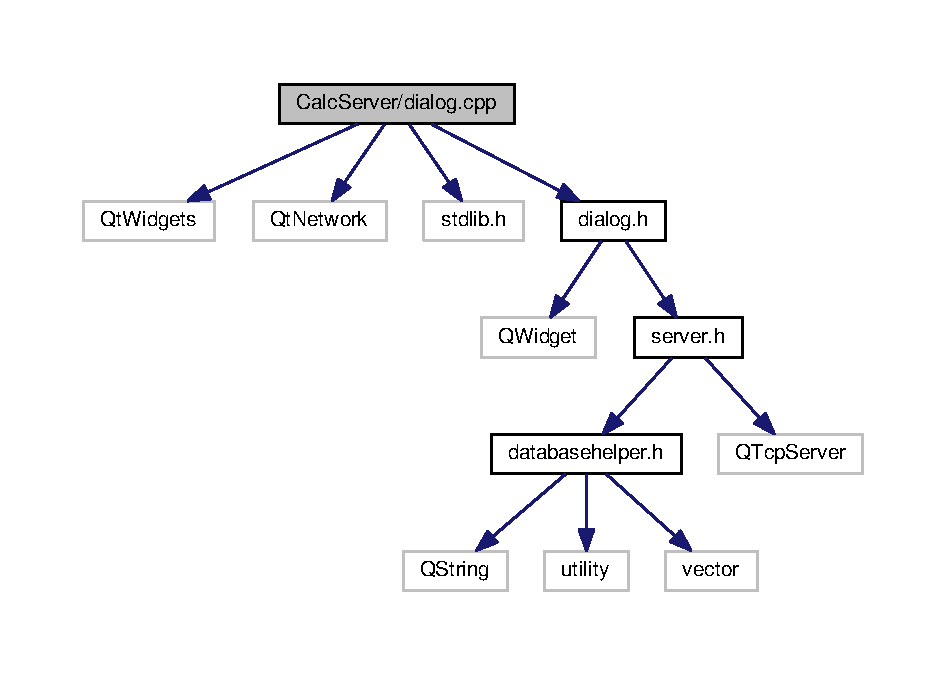
\includegraphics[width=350pt]{dd/d0b/dialog_8cpp__incl}
\end{center}
\end{figure}


\subsection{Detailed Description}
Arquivo contendo a implementação da Classe \hyperlink{classDialog}{Dialog}. 
\hypertarget{dialog_8h}{}\section{Calc\+Server/dialog.h File Reference}
\label{dialog_8h}\index{Calc\+Server/dialog.\+h@{Calc\+Server/dialog.\+h}}
{\ttfamily \#include $<$Q\+Widget$>$}\\*
{\ttfamily \#include \char`\"{}server.\+h\char`\"{}}\\*
Include dependency graph for dialog.\+h\+:\nopagebreak
\begin{figure}[H]
\begin{center}
\leavevmode
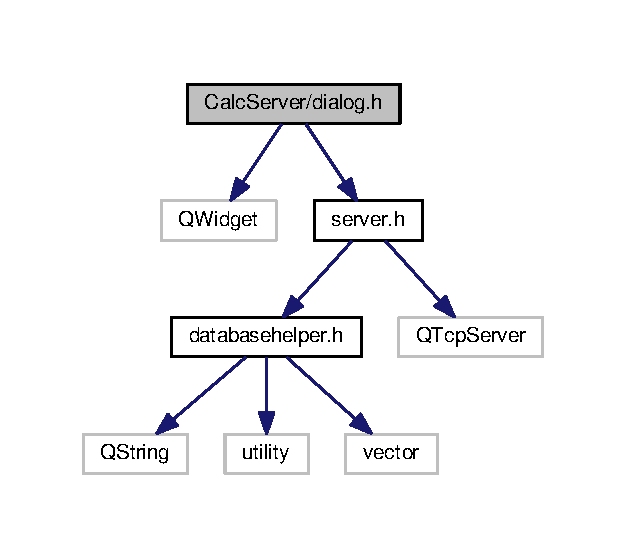
\includegraphics[width=301pt]{d4/d07/dialog_8h__incl}
\end{center}
\end{figure}
This graph shows which files directly or indirectly include this file\+:\nopagebreak
\begin{figure}[H]
\begin{center}
\leavevmode
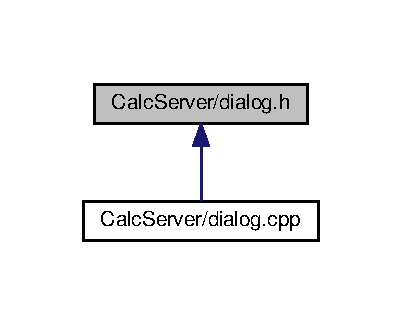
\includegraphics[width=193pt]{d5/d6a/dialog_8h__dep__incl}
\end{center}
\end{figure}
\subsection*{Classes}
\begin{DoxyCompactItemize}
\item 
class \hyperlink{classDialog}{Dialog}
\begin{DoxyCompactList}\small\item\em Classe para exibição dos dados do servidor. \end{DoxyCompactList}\end{DoxyCompactItemize}


\subsection{Detailed Description}
Arquivo contendo a declaração da Classe \hyperlink{classDialog}{Dialog}. 
\hypertarget{server_8cpp}{}\section{Calc\+Server/server.cpp File Reference}
\label{server_8cpp}\index{Calc\+Server/server.\+cpp@{Calc\+Server/server.\+cpp}}
{\ttfamily \#include \char`\"{}server.\+h\char`\"{}}\\*
{\ttfamily \#include \char`\"{}workerthread.\+h\char`\"{}}\\*
{\ttfamily \#include \char`\"{}databasehelperimpl.\+h\char`\"{}}\\*
Include dependency graph for server.\+cpp\+:\nopagebreak
\begin{figure}[H]
\begin{center}
\leavevmode
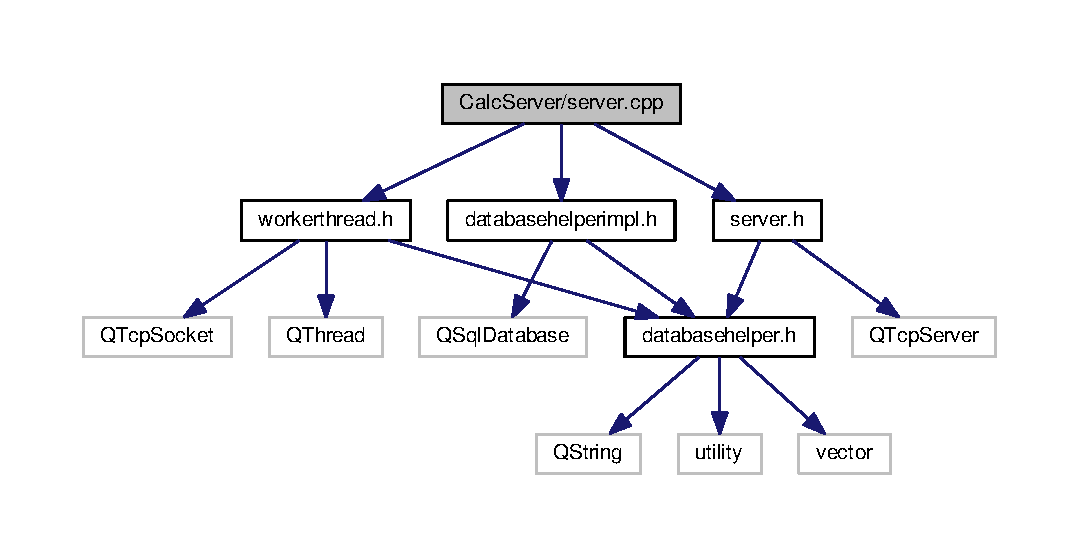
\includegraphics[width=350pt]{d4/d48/server_8cpp__incl}
\end{center}
\end{figure}


\subsection{Detailed Description}
Arquivo contendo a implementação da Classe \hyperlink{classServer}{Server}. 
\hypertarget{server_8h}{}\section{Calc\+Server/server.h File Reference}
\label{server_8h}\index{Calc\+Server/server.\+h@{Calc\+Server/server.\+h}}
{\ttfamily \#include \char`\"{}databasehelper.\+h\char`\"{}}\\*
{\ttfamily \#include $<$Q\+Tcp\+Server$>$}\\*
Include dependency graph for server.\+h\+:\nopagebreak
\begin{figure}[H]
\begin{center}
\leavevmode
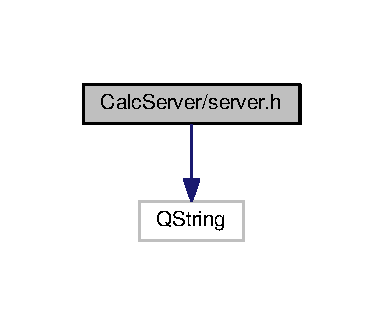
\includegraphics[width=301pt]{d7/d55/server_8h__incl}
\end{center}
\end{figure}
This graph shows which files directly or indirectly include this file\+:\nopagebreak
\begin{figure}[H]
\begin{center}
\leavevmode
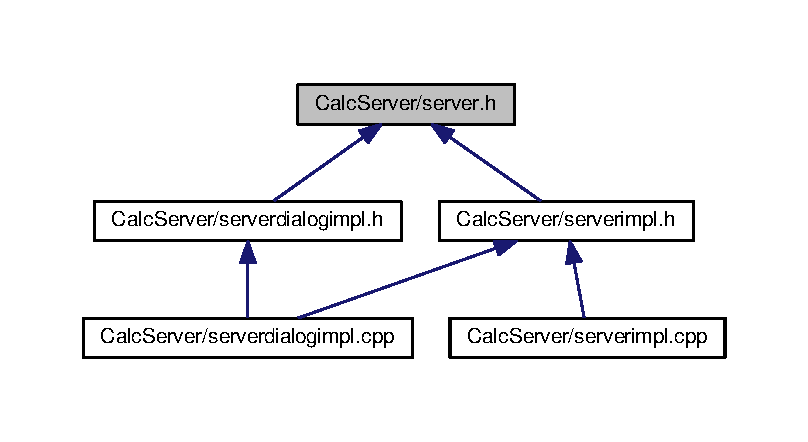
\includegraphics[width=320pt]{d7/d69/server_8h__dep__incl}
\end{center}
\end{figure}
\subsection*{Classes}
\begin{DoxyCompactItemize}
\item 
class \hyperlink{classServer}{Server}
\begin{DoxyCompactList}\small\item\em Clase para gerenciamento de servidor T\+CP. \end{DoxyCompactList}\end{DoxyCompactItemize}


\subsection{Detailed Description}
Arquivo contendo a declaração da Classe \hyperlink{classServer}{Server}. 
\hypertarget{workerthread_8cpp}{}\section{Calc\+Server/workerthread.cpp File Reference}
\label{workerthread_8cpp}\index{Calc\+Server/workerthread.\+cpp@{Calc\+Server/workerthread.\+cpp}}
{\ttfamily \#include \char`\"{}workerthread.\+h\char`\"{}}\\*
{\ttfamily \#include $<$Qt\+Network$>$}\\*
{\ttfamily \#include $<$Q\+Debug$>$}\\*
{\ttfamily \#include $<$Q\+Data\+Stream$>$}\\*
{\ttfamily \#include $<$Q\+Sql\+Database$>$}\\*
{\ttfamily \#include $<$Q\+Sql\+Query$>$}\\*
{\ttfamily \#include $<$Q\+Sql\+Error$>$}\\*
{\ttfamily \#include $<$Q\+Json\+Object$>$}\\*
{\ttfamily \#include $<$Q\+Json\+Document$>$}\\*
Include dependency graph for workerthread.\+cpp\+:\nopagebreak
\begin{figure}[H]
\begin{center}
\leavevmode
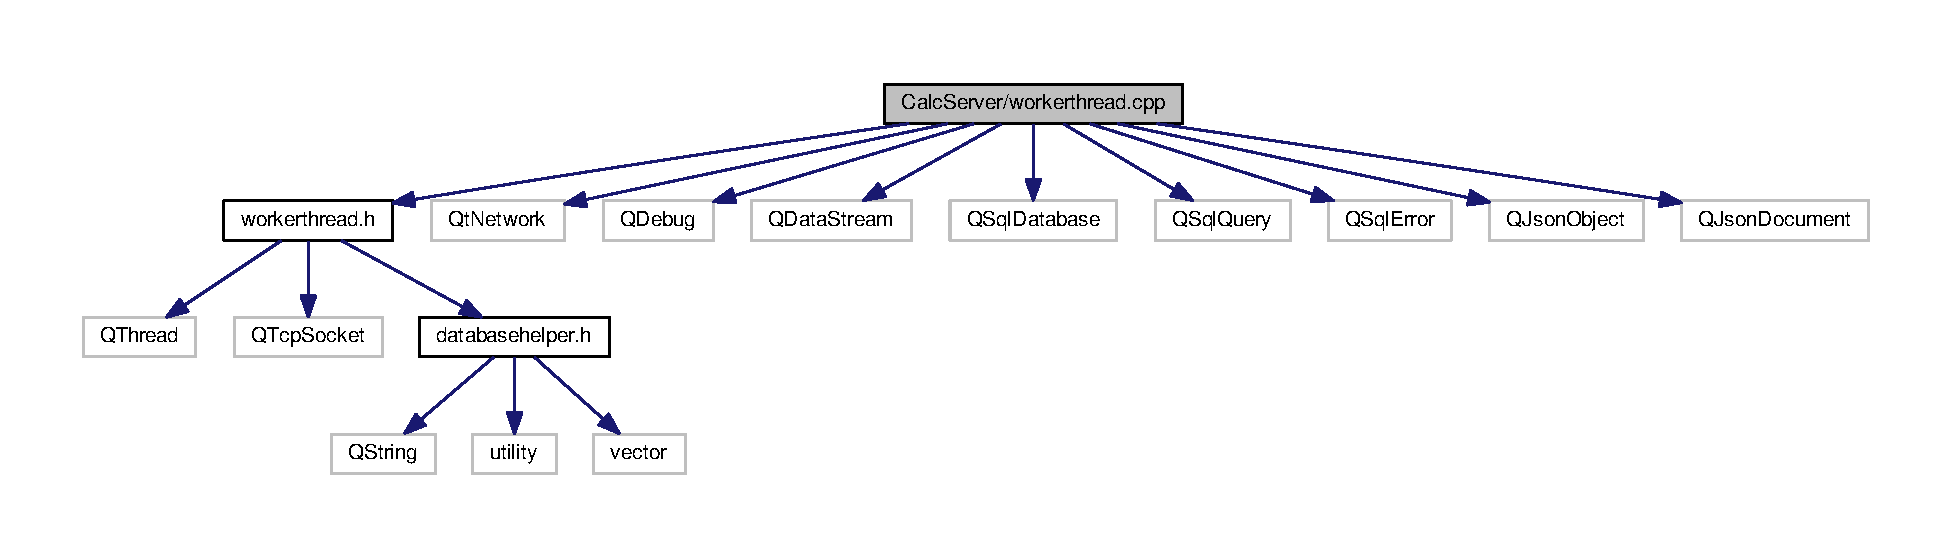
\includegraphics[width=350pt]{da/d6e/workerthread_8cpp__incl}
\end{center}
\end{figure}
\subsection*{Macros}
\begin{DoxyCompactItemize}
\item 
\#define \hyperlink{workerthread_8cpp_ad72dbcf6d0153db1b8d8a58001feed83}{D\+E\+B\+UG}
\end{DoxyCompactItemize}


\subsection{Detailed Description}
Arquivo contendo a implementação da Classe \hyperlink{classWorkerThread}{Worker\+Thread}. 

\subsection{Macro Definition Documentation}
\index{workerthread.\+cpp@{workerthread.\+cpp}!D\+E\+B\+UG@{D\+E\+B\+UG}}
\index{D\+E\+B\+UG@{D\+E\+B\+UG}!workerthread.\+cpp@{workerthread.\+cpp}}
\subsubsection[{\texorpdfstring{D\+E\+B\+UG}{DEBUG}}]{\setlength{\rightskip}{0pt plus 5cm}\#define D\+E\+B\+UG}\hypertarget{workerthread_8cpp_ad72dbcf6d0153db1b8d8a58001feed83}{}\label{workerthread_8cpp_ad72dbcf6d0153db1b8d8a58001feed83}
Flag demarcando se as mensagens de debug devem ou não serem exibidas. 
\hypertarget{workerthread_8h}{}\section{Calc\+Server/workerthread.h File Reference}
\label{workerthread_8h}\index{Calc\+Server/workerthread.\+h@{Calc\+Server/workerthread.\+h}}
{\ttfamily \#include $<$Q\+Object$>$}\\*
Include dependency graph for workerthread.\+h\+:\nopagebreak
\begin{figure}[H]
\begin{center}
\leavevmode
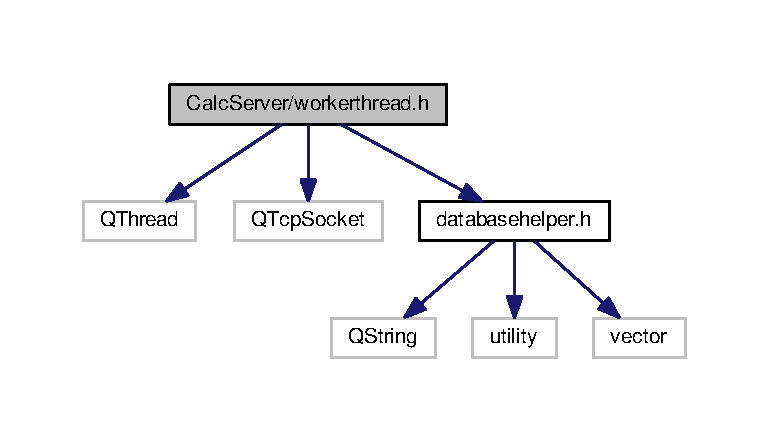
\includegraphics[width=213pt]{d2/d00/workerthread_8h__incl}
\end{center}
\end{figure}
This graph shows which files directly or indirectly include this file\+:\nopagebreak
\begin{figure}[H]
\begin{center}
\leavevmode
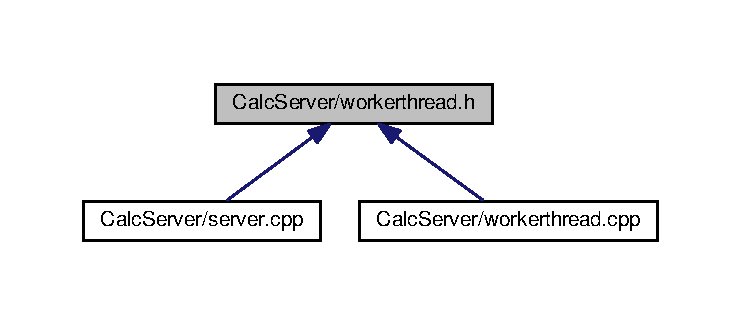
\includegraphics[width=350pt]{d8/d72/workerthread_8h__dep__incl}
\end{center}
\end{figure}
\subsection*{Classes}
\begin{DoxyCompactItemize}
\item 
class \hyperlink{classWorkerThread}{Worker\+Thread}
\begin{DoxyCompactList}\small\item\em Interface para thread de trabalho auxiliar. \end{DoxyCompactList}\end{DoxyCompactItemize}


\subsection{Detailed Description}
Arquivo contendo a declaração da Interface \hyperlink{classWorkerThread}{Worker\+Thread}. 
%--- End generated contents ---

% Index
\backmatter
\newpage
\phantomsection
\clearemptydoublepage
\addcontentsline{toc}{chapter}{Index}
\printindex

\end{document}
